%%====================================================================%%
%%                AKADEMIA GÓRNICZO-HUTNICZA W KRAKOWIE
%%                    WYDZIAŁ MATEMATYKI STOSOWANEJ
%%                          PRACA MAGISTERSKA
%%
%%       Autor : ----
%% Specjalność : ----
%%   Nr albumu : ----
%%    Promotor : ----
%%  Data (wer) : DD.MM.YYYY ...
%%
%%--------------------------------------------------------------------%%
%%
%%
%% ---------------
%%   PLIK GŁÓWNY
%% ---------------
%%
\documentclass[man,mfi|min|mpt|mok|mub|mza|miz|bsp]{mgrwms}

%%
%  Szablon dla kodowania UTF-8 przygotowany z pierwotnego szablonu
%  przy pomocy programu Gżegżółka 5.51.03 (www.gzegzolka.com)
%
%  Obowiązkowe opcje klasy:
%  - woman|man : wersja odpowiednio dla Pań i Panów,
%  - mfi|min|mpt|mok|mub|mza|miz|bsp : specjalności według skrótów:
%      * mfi :  Matematyka finansowa
%      * min :  Matematyka w informatyce
%      * mpt :  Matematyka w naukach technicznych i przyrodniczych
%      * mok :  Matematyka obliczeniowa i komputerowa
%      * mub :  Matematyka ubezpieczeniowa
%      * mza :  Matematyka w zarządzaniu
%      * miz :  Matematyka w informatyce i zarządzaniu
%      * bsp :  Bez specjalności
%  (opis pozostałych opcji znajduje się w dokumentacji 'UserGuide.pdf')
%%
%% ------- PAKIETY ------- %%
%%
\usepackage[utf8]{inputenc}      % kodowanie UTF-8
% \usepackage{amsmath}           % łatwiejszy skład matematyki
% \usepackage{amssymb}
% \usepackage{setspace}          % zmiana interlinii (np. 1,5 wiersza odstępu)
% \usepackage{makeidx}           % odkomentować, jeśli dołączony jest indeks
%
%  <... pozostale pakiety wedle uznania ...>
%
\usepackage{polski}         % pakiet polonizacyjny

\newcommand{\source}[1]{{Źródło: {#1}} }

\usepackage{color}
\usepackage{graphicx}
\usepackage{hyperref}
\usepackage{listings}

\usepackage{amsmath}
\usepackage{nccmath}

\usepackage{dirtree}
\usepackage{float}

\lstset{
language=Python,
basicstyle=\small\sffamily,
numbers=left,
numberstyle=\tiny,
frame=tb,
%columns=fullflexible,
columns=fixed,
showstringspaces=false
}

%\titleclass{\subsubsubsection}{straight}[\subsection]

%\newcounter{subsubsubsection}[subsubsection]
%\renewcommand\thesubsubsubsection{\thesubsubsection.\arabic{subsubsubsection}}
%\renewcommand\theparagraph{\thesubsubsubsection.\arabic{paragraph}} % optional; useful if paragraphs are to be numbered

%\titleformat{\subsubsubsection}
%  {\normalfont\normalsize\bfseries}{\thesubsubsubsection}{1em}{}
%\titlespacing*{\subsubsubsection}
%{0pt}{3.25ex plus 1ex minus .2ex}{1.5ex plus .2ex}

\makeatletter
\renewcommand\paragraph{\@startsection{paragraph}{5}{\z@}%
  {3.25ex \@plus1ex \@minus.2ex}%
  {-1em}%
  {\normalfont\normalsize\bfseries}}
\renewcommand\subparagraph{\@startsection{subparagraph}{6}{\parindent}%
  {3.25ex \@plus1ex \@minus .2ex}%
  {-1em}%
  {\normalfont\normalsize\bfseries}}
\def\toclevel@subsubsubsection{4}
\def\toclevel@paragraph{5}
\def\toclevel@paragraph{6}
\def\l@subsubsubsection{\@dottedtocline{4}{7em}{4em}}
\def\l@paragraph{\@dottedtocline{5}{10em}{5em}}
\def\l@subparagraph{\@dottedtocline{6}{14em}{6em}}
\makeatother

\setcounter{secnumdepth}{4}
\setcounter{tocdepth}{4}


\graphicspath{ {/home/lukas/mgr/MData/mData_latex/schema/szablon/images/} }
% \usepackage[T1]{fontenc}  % lub z opcją 'QX', wymagane dla pakietu 'lmodern'
% \usepackage{lmodern}      % zalecane czcionki LModern
%%
%  Dodatkowe polecenia które trzeba umieścić w preambule:
%
% \makeindex  % jeśli dołączony jest indeks (nieobowiązkowy)
% \includeonly{...,...,...,...}  % dla warunkowej kompilacji
%%
%% BiBTeX (opcjonalnie)
% \bibliographystyle{ddabbrv}  % lub np. plabbrv, plalpha, plplain ...
% \nocite{*}
%%
%%
\begin{document}
%%
%%
%% ---------------
%%   NASZE MAKRA
%% ---------------
%%
%  Miejsce na nasze makra. Innym sposobem może być
%  umieszczenie ich w osobnym pliku i wczytanie poleceniem \input{----}
%%
%%
%% ---------------------------------
%%   METRYCZKA PRACY i SPIS TREŚCI
%% ---------------------------------
%%
\title{Analiza danych giełdowych przy pomocy narzędzi dostępnych w pakiecie scikit-learn}
\author{Łukasz Połoń}
\promotor{dr inż. Piotr Błaszyński}
\nralbumu{24942}
\slowakluczowe{Python, Scikit-learn, Giełda Papierów Wartościowych, Kivy, Matplotlib, Pandas, Analiza regresji}
\keywords{Python, Scikit-learn, Stock Market, Kivy, Matplotlib, Pandas, Regression analysis}
\maketitle
%%
%%
\tableofcontents
%%
%%
%% ----------------------
%%   STRESZCZENIA PRACY
%% ----------------------
%%
%% ------- POLSKIE ------- %%
%%
\begin{streszczenie}
%%
Przykładowe streszczenie i test polskich znaków: ąśćżźłóęą

%
%  <Treść streszczenia po polsku>
%
%%
\end{streszczenie}
%%
%% ------- ANGIELSKIE ------- %%
%%
\begin{abstract}
%%
%
%  <Treść streszczenia po angielsku>
%
%%
\end{abstract}
%%
%% ------- PODZIĘKOWANIA ------- %%
%%
%  <Jeśli zachodzi taka potrzeba, można dodać tutaj tekst podziękowania,
%   dedykacji itp.>
% \newpage
% \thispagestyle{empty}
%  <Treść podziękowania z odpowiednim formatowaniem>
%%
%%
%% ----------------------
%%   GŁÓWNY TEKST PRACY
%% ----------------------
%%
%% ------- WSTĘP ------- %%
%%
\begin{wstep}[Wprowadzenie]  % ew. np. \begin{wstep}[Wprowadzenie]
%%
Giełda Papierów Wartościowych jest to instytucja, która prowadzi działalność w zakresie organizacji obrotu papierami wartościowymi i instrumentami finansowymi\cite{gpw}.
W praktyce spełnia ona rolę pośrednika finansowego pomiędzy kupującym, a sprzedającym papiery wartościowe.
Dane generowane przez giełdę poddawane są ciągłym analizom, w szczególności w celu dostarczenia informacji potrzebnych do właściwego zarządzania kapitałem.\\
Istnieją dwie główne metody analizy danych giełdowych: analiza fundamentalna i analiza techniczna\cite{basics_of_tech_analysis}.
Pierwsza z nich polega na analizie faktycznej kondycji finansowej podmiotu, podczas gdy druga ma za zadanie prognozowanie przyszłych wartości wskaźników na podstawie zebranych danych.\\

Temat tej pracy podejmuje opisanie i przeprowadzenie wybranych metod analitycznych dostępnych w pakiecie scikit-learn. Pakiet ten jest biblioteką języka programowania Python umożliwiającą wysokopoziomowe przetwarzanie danych.
Udostępnia wiele algorytmów klasyfikacji, regresji oraz uczenia maszynowego, które mogą zostać wykorzystane do przeprowadzania obliczeń między innymi na potrzeby analizy technicznej, której to elementy zostaną tutaj przedstawione.

%%
\end{wstep}
%%
\input{chapter_1}

%% ------- ROZDZIAŁ 2 ------- %%

\chapter{Zastosowanie języka programowania Python w obliczeniach analitycznych}
Python jest językiem programowania wysokiego poziomu, charakteryzujący się przede wszystkim wysoką klarownością i czytelnością kodu.
Jest to język interpretowany, co w odróżnieniu od języków kompilowanych pozwala na bardzo szybkie tworzenie i testowanie kodu.
Wadą tego rozwiązania jest niestety spadek wydajności oraz zwiększone zużycie pamięci i procesora, jednak zastosowania praktyczne Pythona zazwyczaj pozwalają na poniesienie tego typu kosztów.\\

Python został stworzony w 1989 roku przez Guido van Rossum, a do dzisiaj rozwijany jest jako projekt Open Source i zarządzany przez organizację non-profit Python Software Foundation.
Jego specyficzna struktura oraz cechy takie jak dynamiczne typowanie, automatyczne zarządzanie pamięcią, przenośność, czy duża czytelność i prostota kodu, 
umożliwiają bardzo szybkie wytwarzanie i utrzymywanie aplikacji.\\

Biblioteka standardowa języka Python zawiera wiele użytecznych modułów i gotowych rozwiązań, które wspomagają szybką i efektywną implementację kodu.
Ponadto dostępny jest \textit{Python Package Index} (PyPI) - zbiór paczek zewnętrznych, tworzonych przez niezależnych programistów, dystrybuowanych na licencjach Open Source.
Dzięki takiej mnogości pakietów i modułów język Python może być wykorzystywany w wielu projektach, łącząc różne technologie i dziedziny informatyki.
Jednym z przykładów wykorzystania tego języka jest tworzenie aplikacji internetowych za pomocą frameworku Django.
Łączy on ze sobą różne technologie wykorzystywane przy tworzeniu serwisów internetowych, zapewniając bardzo dobry mechanizm back-endowy oraz wygodne środowisko.\\

Ze względu na wyżej wymienione cechy Python znalazł również zastosowanie w analityce i analizie danych, włączając w to analizę danych statystycznych i giełdowych, a także we wspomaganiu obliczeń matematycznych.


\section{Cechy charakterystyczne języka Python}
Podstawową charakterystyczną cechą języka Python jest fakt, iż nie jest on kompilowany lecz interpretowany, czyli tłumaczony do wykonywalnego kodu maszynowego lub kodu pośredniego.
Dzięki użyciu interpretera w konsoli systemowej można bezpośrednio wykonywać kod Pythona w czasie rzeczywistym.


\begin{lstlisting}
Python 2.7.12 (default, Nov 20 2017, 18:23:56) 
[GCC 5.4.0 20160609] on linux2
Type "help", "copyright", "credits" or "license" for more information. 
>>> from sklearn import datasets
>>> 
>>> iris = datasets.load_iris()
>>> digits = datasets.load_digits()
>>> digits.data
array([[  0.,   0.,   5., ...,   0.,   0.,   0.],
       [  0.,   0.,   0., ...,  10.,   0.,   0.],
       [  0.,   0.,   0., ...,  16.,   9.,   0.],
       ..., 
       [  0.,   0.,   1., ...,   6.,   0.,   0.],
       [  0.,   0.,   2., ...,  12.,   0.,   0.],
       [  0.,   0.,  10., ...,  12.,   1.,   0.]])
>>>
>>>
\end{lstlisting}

Pozwala to na bardzo szybkie testowanie niewielkich fragmentów kodu, użycia bibliotek, a także przeprowadzanie testowych obliczeń.
Jest to również doskonałe narzędzie do sprawdzania i dostosowywania środowiska, w szczególności gdy użyte zostaje symulowane środowisko - program \textit{virtualenv}, 
który instaluje wybraną wersję interpretera we wskazanym katalogu i umożliwia instalowanie bibliotek niezależnie od tych, które zainstalowane są w systemie.\\

Kolejną wartą uwagi cechą języka Python jest jego składnia. W odróżnieniu od języków takich jak na przykład Java czy C++, w Pythonie zastosowano tak zwane dynamiczne typowanie.
Oznacza to, że podczas definiowania zmiennych nie określa się ich typu. Jest to możliwe, ponieważ w języku Python każdy element, na przykład funkcja, klasa czy też struktura danych jest obiektem.
Obiekt ten ma z góry zdefiniowany typ, więc przypisanie jego referencji do konkretnej zmiennej pomaga go w ten sposób określić.
\begin{lstlisting}
  Python 2.7.12 (default, Nov 20 2017, 18:23:56) 
  [GCC 5.4.0 20160609] on linux2
  Type "help", "copyright", "credits" or "license" for more information.
  >>> variable_one = 44
  >>> type(variable_one)
  <type 'int'>
  >>> 
  >>> variable_one = 'text'
  >>> type(variable_one)
  <type 'str'>
  >>> 
\end{lstlisting}

Jedną z najbardziej użytecznych cech Pythona jest zastosowanie elementów programowania funkcyjnego. Elementami takimi są przykładowo wyrażenia \textit{lambda}, oraz \textit{list comprehension} i \textit{dict comprehension}.\\

Wyrażenia \textit{lambda} pozwalają na stworzenie i przypisanie do zmiennej krótkiej funkcji, która jest w stanie przyjmować argumenty oraz zwracać wartości.
Znajduje to zastosowanie w przypadkach, które wymagają wielokrotnego wykorzystania danego fragmentu kodu, a użycie ich skraca znacznie ilość wypisanych poleceń.
Pozwala to uniknąć tworzenia wielu krótkich funkcji lub metod poza obecnie wykorzystywaną przestrzenią, co często wpływa pozytywnie przede wszystkim na czytelność kodu.\\

Wyrażenia \textit{list comprehension} oraz \textit{dict comprehension} wykorzystywane są do szybkiego tworzenia odpowiednio list oraz słowników.
W swojej konstrukcji zawierają pętlę \textit{For}, która iteruje po wskazanej strukturze, na przykład liście, zwracając w każdym kroku jeden jej element.
Element ten może być sprawdzony warunkiem wbudowanym w strukturę, oraz następnie zmieniony i wbudowany w nową listę lub słownik.

\begin{lstlisting}
  Python 2.7.12 (default, Nov 20 2017, 18:23:56) 
  [GCC 5.4.0 20160609] on linux2
  Type "help", "copyright", "credits" or "license" for more information. 
  >>> test_lambda = lambda x: x+5
  >>> test_lambda(10)
  15
  >>> 
  >>> test_list = [1, 2, 3, 4, 5]
  >>> 
  >>> list_comprehension = [x+5 for x in test_list]
  >>> list_comprehension
  [6, 7, 8, 9, 10]
  >>> 
  >>> dict_comprehension = {x: x+1 for x in test_list}
  >>> dict_comprehension
  {1: 2, 2: 3, 3: 4, 4: 5, 5: 6}
  >>> 
\end{lstlisting}

Naturalnie, natura i składnia języka Python jest o wiele bardziej różnorodna, a przedstawione przykłady odzwierciedlają jedynie namiastkę jego możliwości.
Należałoby wspomnieć tutaj między innymi o posługiwaniu się choćby wbudowanymi strukturami danych, wykorzystaniu programowania orientowanego obiektowo oraz typowych dla niego elementach.
Niemniej jednak, biorąc pod uwagę temat niniejszej pracy, którym jest przedstawienie możliwości biblioteki \textit{Scikit-learn}, wyżej wymienione podstawy uzupełnione późniejszymi wyjaśnieniami powinny wystarczyć aby w pełni zrozumieć naturę problemu.




\section{Python w obliczeniach analitycznych}
Język programowania Python jest bardzo dobrym narzędziem wspomagającym obliczenia analityczne.
Cechy tego języka zapewniają skoncentrowanie się na bezpośrednim podejściu do problemu tworzenia algorytmów i modeli, minimalizując czas projektowania od podstaw skomplikowanych algorytmów pomocniczych.
Jednak największą zaletą tego języka jest dostępność wielu bibliotek z gotowymi rozwiązaniami, które mogą zostać wykorzystane do sprawnej implementacji modeli analitycznych.
Podstawowymi bibliotekami wspomagającymi przeprowadzanie obliczeń matematycznych są \textit{NumPy} i \textit{SciPy}.\\

Pierwsza z nich dostarcza przede wszystkim obiekty wielowymiarowych list oraz szereg metod i funkcji umożliwiających szybką manipulację, przetwarzanie i sortowanie.
Zawiera także zestaw metod pozwalających na przeprowadzanie podstawowych działań statystycznych i matematycznych\cite{numpy_ug}. Stosowana jest w wielu innych bibliotekach analitycznych, na przykład w pakiecie \textit{Scikit-learn}.\\

Podstawową różnicą pomiędzy obiektami \textit{array} z pakietu \textit{NumPy}, a wbudowanymi listami języka Python jest fakt, iż podczas tworzenia obiektu ustala się stały rozmiar struktury, 
a każde zwiększenie tego rozmiaru powoduje powstanie nowego obiektu i usunięcie poprzedniego.
\begin{lstlisting}
 >>> python_list = [1, 2, 3, 4]
 >>> before_append = id(python_list)
 >>> python_list.append(5)
 >>> python_list
 [1, 2, 3, 4, 5]
 >>> after_append = id(python_list)
 >>> print(before_append, after_append)
 (140635439293360, 140635439293360)
 >>> print(before_append == after_append)
 True
 >>> 
 >>> 
 >>> import numpy as np
 >>> np_array = np.zeros(shape=(1, 4))
 >>> np_array
 array([[ 0.,  0.,  0.,  0.]])
 >>> before_resize = id(np_array)
 >>> np_array = np.resize(np_array, (1, 5))
 >>> np_array
 array([[ 0.,  0.,  0.,  0.,  0.]])
 >>> after_resize = id(np_array)
 >>> print(before_resize, after_resize)
 (139910114654128, 139910001813664)
 >>> print(before_resize == after_resize)
 False
 >>> 
\end{lstlisting}

Powyższa cecha obiektów biblioteki \textit{NumPy} oznacza, że wykonywanie operacji na takich obiektach powinno być bardziej skuteczne pod względem czasu ich przeprowadzania.
Jednakże wielokrotne przebudowywanie struktury obiektu wiąże się z bardzo dużym zużyciem pamięci, dlatego polecane jest stosowanie konwersji i tworzenie obiektów dopiero w momencie, kiedy dane są skompletowane i gotowe do przetwarzania\cite{numpy_ug}.\\

Biblioteka \textit{SciPy} zbudowana jest na podstawie biblioteki \textit{NumPy} i rozszerza ją o wiele algorytmów analizy danych.
Elementami składowymi tej biblioteki są między innymi\cite{numpy_ug}:
\begin{itemize}
 \item \textbf{cluster} - algorytmy klastrowania
 \item \textbf{linalg} - algebra liniowa
 \item \textbf{signal} - przetwarzanie sygnałów
 \item \textbf{stats} - funkcje i algorytmy statystyczne\\
\end{itemize}

Funkcjonalność biblioteki jest bardzo szeroka, dzięki czemu znajduje ona zastosowanie w wielu projektach, a także jest ona częścią składową innych bibliotek analitycznych języka Python.
Przykładową metodą należącą do biblioteki \textit{stats} jest \textit{linregress}, która umożliwia przeprowadzenie regresji liniowej dla wskazanych danych.
\begin{lstlisting}
 >>> from scipy import stats
 >>> import numpy as np
 >>>
 >>> data_x = np.random.random_integers(1, 99, 10)
 >>> data_y = np.random.random_integers(1, 99, 10)
 >>> data_x
 array([72, 45, 69, 52, 93, 14, 80, 14, 13,  5])
 >>> data_y
 array([37, 90, 19,  7, 95, 89, 88, 94, 81, 19])
 >>>
 >>> slope, intercept, r_value,
     p_value, std_err = stats.linregress(data_x, data_y)
 >>> print(slope, intercept, r_value, p_value, std_err)
 (-0.033350664784966184, 63.424125380672955,
  -0.029541780200591877, 0.93543372355182242, 0.39896357644710517)
 >>> 
\end{lstlisting}

\section{Pakiet Scikit-learn}

\subsection{Cel i przeznaczenie pakietu}
Biblioteka \textit{Scikit-learn} zawiera zestaw zaawansowanych narzędzi stosujących uczenie maszynowe do analizy danych w języku Python.
Dystrybuowana jest na licencji BSD, która pozwala na modyfikowanie i rozprowadzanie kodu źródłowego, a nawet na włączanie go do produktów komercyjnych pod warunkiem umieszczenia w dokumentacji odpowiednich adnotacji dotyczących autorów.
Dzięki temu zaliczana jest do wolnego oprogramowania, które rozwijane jest przez społeczność kontrybutorów.
Większa część kodu stworzona jest bezpośrednio w języku Python, lecz niektóre elementy takie jak na przykład implementacje SVM oraz modeli liniowych oparte są na bibliotekach języka C++, odpowiednio LibSVM oraz LibLinear\cite{scikit_article}.\\

Podstawowym założeniem twórców biblioteki jest priorytetyzacja utrzymywania jakości i czytelności kodu, ponad implementację bardzo wielu funkcji\cite{scikit_article}.
Dodatkowo rozwijana jest wysokiej jakości kompleksowa dokumentacja, co razem stanowi bardzo dobrą bazę do rozwijania całego projektu przez wielu niezależnych deweloperów i wydawania stabilnych wersji produktu.
Scikit-learn bazuje na trzech bibliotekach języka Python: \textit{NumPy}, \textit{SciPy} i \textit{Matplotlib}. Stanowią one wymagania systemowe, niezbędne do poprawnego działania pakietu.\\

W pakiecie \textit{Scikit-learn} algorytmy podzielone są na algorytmy uczenia z nadzorem oraz algorytmy uczenia bez nadzoru\cite{scikit_doc}.
Pierwsze z nich opierają się o podział danych na uczące i testowe, gdzie dane uczące zawierają przykładowe oczekiwane wartości na podstawie których budowany jest model.
W zestawie algorytmów uczenia nadzorowanego znaleźć można między innymi\cite{scikit_doc}:
\begin{itemize}
 \item Ogólne modele liniowe
 \item Liniową i kwadratową analizę dyskryminacyjną
 \item Regresję grzbietową (KRR)
 \item Maszynę wektorów nośnych (SVM)
 \item Algorytm k najbliższych sąsiadów
 \item Proces Gaussa
 \item Naiwny klasyfikator Bayesa
 \item Drzewa decyzyjne\\
\end{itemize}

Algorytmy uczenia bez nadzoru w pakiecie \textit{Scikit-learn}, dla których dane uczące nie posiadają żadnych wartości odniesienia, możemy natomiast podzielić między innymi na:
\begin{itemize}
 \item Klasteryzację
 \item Estymację kowariancji
 \item Nieliniową redukcję przestrzenną\\
\end{itemize}

W niniejszej pracy zastosowane zostały algorytmy uczenia z nadzorem.

\subsection{Ogólne modele liniowe}
W pakiecie \textit{Scikit-learn} przedstawione zostały algorytmy regresji, w których oczekiwane wartości docelowe są liniową kombinacją wartości wejściowych.
Podstawę stanowi równanie regresji:
\begin{ceqn}
\begin{align}
\hat{y} = \omega_{0} + \omega_{1}X_{1} + \omega_{2}X_{2} + ... + \omega_{p}X_{k}
\end{align}
\end{ceqn}

Wektor $\omega = (\omega_{1}, ..., \omega_{p})$ jest utożsamiany z parametrem \textit{coef\_}, a wyraz wolny $\omega_{0}$ z parametrem \textit{intercept\_} \cite{scikit_doc}.\\

\newpage

Regresja liniowa w pakiecie \textit{Sciki-learn} dostępna jest poprzez obiekt \textbf{LinearRegression}.
Parametry, jakie przyjmuje ten obiekt w momencie inicjalizacji to\cite{scikit_doc}:
\begin{itemize}
 \item \textit{fit\_intercept}: boolean, optional, default True
 \item \textit{normalize}: boolean, optional, default False
 \item \textit{copy\_X}: boolean, optional, default True
 \item \textit{n\_jobs}: int, optional, default 1\\
\end{itemize}

Parametr \textit{fit\_intercept} przyjmuje wartości typu boolean, a jego domyślna wartość wynosi \textit{True}.
W takim wypadku przed procesem dopasowania modelu obliczany jest punkt przecięcia z osią \textit{y} dla modelu.
Jeśli przed procesem dopasowywania modelu dokonano normalizacji danych, parametr może zostać ustawiony wartością \textit{False}.\\

Parametr \textit{normalize} jest flagą uwzględniającą lub pomijającą wstępną normalizację danych.
Przyjmuje wartości typu boolean i domyślnie jest ustawony na \textit{False} i jest ignorowany, gdy parametr \textit{fit\_intercept} jest ustawiony wartością \textit{False}.
Jeśli przed dokonaniem dopasowania modelu nie została przeprowadzona normalizacja danych, ustawienie tego parametru na \textit{True} spowoduje ich przetworzenie.\\

Parametr \textit{copy\_X} jest odpowiedzialny za ustawienie flagi kopiowania, bądź nadpisywania wartości X. Domyślnie ustawiony jest na wartość \textit{True}, więc w tym przypadku podane dane X są kopiowane.\\

Parametr \textit{n\_jobs} określa ilość procesorów, które będą użyte do przetwarzania danych. Przyjmuje wartości typu integer, a domyślnie ustawiony jest wartością 1.
Jeśli podana zostanie wartość -1, wykorzystane zostaną wszystkie dostępne procesory. Znajduje on praktyczne zastosowanie przy przetwarzaniu dużych zbiorów danych, skracając czas wykonania obliczeń.\\

\begin{lstlisting}
 >>> from sklearn.linear_model import LinearRegression
 >>> LinearRegression()
 LinearRegression(copy_X=True, fit_intercept=True, n_jobs=1,
                  normalize=False)
 >>>
\end{lstlisting}\\


Obiekt udostępnia następujące metody:
\begin{itemize}
 \item \textit{fit}: dopasowanie modelu liniowego
 \item \textit{get\_params}: pobranie parametrów estymacji
 \item \textit{predict}: predykcja na podstawie modelu liniowego
 \item \textit{score}: współczynnik determinacji $R^2$
 \item \textit{set\_params}: ustawienie parametrów estymacji\\
\end{itemize}

\newpage

Metoda \textit{fit()} jest odpowiedzialna za dopasowanie modelu dla podanych danych. Jako argumenty przyjmuje dane testowe X, które powinny być strukturą definiowaną typem \textit{numpy.ndarray}. Przykładowo:
\begin{lstlisting}
 >>> X = np.asarray([x for x in range(5)])
 >>> X
 array([0, 1, 2, 3, 4])
 >>> X.reshape(-1, 1)
 array([[0],
        [1],
        [2],
        [3],
        [4]])
 >>>
\end{lstlisting}
Wartości y, jako kolejny argument przyjmowany przez funkcję, powinny być zgodne typem z wartościami X, lecz ich postać powinna być macierzą jednowymiarową.
Ważną informacją jest fakt, iż struktura X oraz struktura y powinny mieć dokładnie ten sam rozmiar. W innym przypadku niemożliwe jest dokonanie dopasowania, a metoda zwraca błąd \textit{ValueError}.
W przypadku danych giełdowych wartości X utożsamiane są przez przekształcone wartości dat kolejnych próbek danych testowych, natomiast wartości y to odpowiadające im ceny akcji lub wielkości wolumenu.\\

Kolejną metodą klasy \textit{LinearRegression} jest \textit{predict()}. Umożliwia ona dokonanie obliczeń predykcji dla podanych danych testowych X, na podstawie dopasowanego przy pomocy metody \textit{fit()} modelu.
Przyjmowane dane testowe powinny być zgodne zarówno typem, jak i formatem struktury z danymi testowymi X użytymi do przeprowadzenia dopasowania modelu metodą \textit{fit()}.

\begin{lstlisting}
 >>> import random
 >>> import numpy as np
 >>> from sklearn.linear_model import LinearRegression
 >>>
 >>> X = np.asarray(range(1, 10))
 >>> X.reshape(-1, 1)
 >>> y = np.asarray(sorted([random.uniform(1.0, 2.0)
                            for x in range(10)]))
 >>> print(y)
 array([ 1.03622622,  1.08102786,  1.15758493,  1.30854005,
         1.43797429,  1.47473032,  1.5770967 ,  1.64707456,
         1.7256157 ,  1.8449893 ])
 >>> X_test = np.asarray(11, 15)
 >>> X_test = X_test.reshape(-1, 1)
 >>>
 >>> linear = LinearRegression()
 >>> linear.fit(X, y)
 LinearRegression(copy_X=True, fit_intercept=True, n_jobs=1,
                  normalize=False)
 >>> linear.predict(X_test)
 array([ 2.02318035,  2.11457948,  2.20597861,  2.29737775])
 >>> linear.predict(X)
 array([ 1.0177899 ,  1.10918903,  1.20058816,  1.2919873 ,
         1.38338643,  1.47478556,  1.56618469,  1.65758382,
         1.74898295,  1.84038209])
 >>>
\end{lstlisting}


\subsection{Nieliniowe modele regresji}
W pakiecie \textit{Scikit-learn} regresja grzbietowa reprezentowana jest przez klasę \textit{KernelRidge}.
Jest ona w istocie połączeniem algorytmu regresji grzbietowej z tak zwanymi funkcjami jądra (kernel functions).
Najważniejszymi parametrami przyjmowanymi przez tą klasę są:
\begin{itemize}
 \item \textit{alpha}: {float, array}
 \item \textit{kernel}: string, default \textit{linear}
 \item \textit{gamma}: float, default None\\
\end{itemize}

Parametr \textit{kernel} może przyjmować wartości nazw funkcji jądra, na przykład: rbf, laplacian, polynomial lub linear. W niniejszej pracy we wszystkich nieliniowych modelach regresji zastosowano funkcję \textit{rbf}.\\

Parametry \textit{alpha} i \textit{gamma} dobierane są dzięki klasie \textit{sklearn.model\_selection.GridSearchCV}, 
która przyjmuje listy parametrów wraz z oryginalnym obiektem regresji i iterując po ich iloczynie kartezjańskim dobiera taką kombinację, która zwraca najlepsze dopasowanie metody \textit{fit{}}.

\begin{lstlisting}
 >>> krr = GridSearchCV(KernelRidge(kernel='rbf'),
                                param_grid={
                         "alpha": [1e0, 0.1, 1e-2, 1e-3],
                         "gamma": np.logspace(-2, 2, 5)
			 })
 >>> >>> krr
GridSearchCV(cv=None, error_score='raise',
	     estimator=KernelRidge(alpha=1, coef0=1, degree=3,
	                           gamma=None, kernel='rbf',
	                           kernel_params=None),
             fit_params={}, iid=True, n_jobs=1,
             param_grid={'alpha': [1.0, 0.1, 0.01, 0.001], 
                         'gamma': array([  1.00000e-02,
                                           1.00000e-01,
                                           1.00000e+00,
                                           1.00000e+01,
                                           1.00000e+02])},
             pre_dispatch='2*n_jobs', refit=True,
             return_train_score=True, scoring=None, verbose=0)
 >>>             
\end{lstlisting}

Pozostałymi, zastosowanymi w pracy metodami regresji nieliniowej są:
\begin{itemize}
 \item Regresja Wektorów nośnych - \textit{sklearn.svm.SVR} - przyjmująca parametry \textit{C} i \textit{epsilon}
 \item Regresja procesu Gaussa - \textit{sklearn.gaussian\_process.GaussianProcessRegressor} - przyjmująca prarmetr \textit{alpha}\\
\end{itemize}

Do przeprowadzenia procesu normalizacji danych może być użyta klasa \textit{StandardScaler} pakietu \textit{Scikit-learn}. 
\begin{lstlisting}
 >>> sc_x = StandardScaler()
 >>> sc_y = StandardScaler()

 >>> sort_dates = sc_x.fit_transform(dates_delta)
 >>> sort_values = sc_y.fit_transform(sort_values)
 
 >>> sort_dates = sc_x.inverse_transform(sort_dates)
 >>> sort_values = sc_y.inverse_transform(sort_values)
 >>>
\end{lstlisting}

Metoda \textit{fit\_transform} utworzonego obiektu klasy \textit{StandardScaler} umożliwia przeprowadzenie normalizacji, natomiast metoda \textit{inverse\_transform} umożliwia powrót do oryginalnych wartości.





%% ------- ROZDZIAŁ 3 ------- %%

\chapter{Przedstawienie aplikacji}
Na potrzeby tej pracy została napisana aplikacja w języku programowania Python w wersji 2.7, która ma za zadanie przedstawić część możliwości pakietu \textit{Scikit-learn} analizując dane giełdowe.
Zastosowany został graficzny interfejs użytkownika (GUI), dzięki któremu jest możliwa szybka zmiana wybranych opcji, oraz dokonywanie wielu analiz bez potrzeby ponownego uruchamiania aplikacji.
Przeznaczeniem aplikacji jest analiza danych, tak więc generowane wyniki zapisywane są we wskazanym przez użytkownika katalogu, a także wyświetlane bezpośrednio w aplikacji.

\section{Podstawowe założenia}
Aplikacja została napisana w modelu orientowanym obiektowo. Starano się zachować wyraźny podział na część biznesową, oraz interfejs użytkownika. W związku z tym struktura katalogów w projekcie wygląda następująco:
\dirtree{%
.1 /. 
.2 /mdata.
.3 /client.
.3 /drivers. 
.4 /config.
.4 /databases.
.3 /gui. 
.4 /buttons.
.4 /items.
.4 /layouts.
.4 /screens.
}

W katalogu \textit{/client} umieszczony został kod odpowiadający za pobieranie danych giełdowych, przeprowadzanie analizy regresji, oraz generowanie wykresów.
Katalog \textit{/drivers} zawiera mechanizmy zapisu i odczytu głównego pliku konfiguracyjnego aplikacji, oraz mechanizm bazodanowy napisany przy pomocy pakietu \textit{SqlAlchemy}.
Ostatni katalog \textit{/gui} zawiera wszystkie elementy graficznego interfejsu użytkownika, w podziale na przyciski, układy, okna oraz pozostałe elementy.

Przeprowadzono analizę kodu dla katalogu \textit{/mdata} programem \textit{pylint}.\\
Według tego raportu kod aplikacji uzyskał ocenę 7.28/10 i zawiera:
\begin{itemize}
 \item 43 zaimplementowane klasy
 \item 199 zaimplementowanych metod
 \item 2 funkcje pozaklasowe
 \item 1707 linii kodu
\end{itemize}


\subsection{Dane giełdowe}

Ze względu na ogromne możliwości pakietu \textit{Scikit-learn}, a także na ograniczenia dotyczące samej konstrukcji aplikacji, poczynione zostały pewne założenia definiujące działanie aplikacji.\\
Główne założenia związane z pobieraniem danych giełdowych:
\begin{itemize}
 \item Dane giełdowe pobierane są na podstawie wcześniej przygotowanej bazy firm giełdy amerykańskiej
 \item Pobieranie danych giełdowych odbywa się za pomocą API \textit{Yahoo Finance}
 \item Rodzaj danych jest determinowany jedynie przez użyte API, a ich zakres wybierany jest poprzez podanie daty początkowej i końcowej
\end{itemize}\\

Zastosowane w pracy API \textit{Yahoo Finance} umożliwia pobieranie danych jedynie w jednej postaci, bez możliwości wyboru lub dodania dodatkowych elementów.
Każde pobranie danych w tym samym zakresie powoduje otrzymanie dokładnie takich samych rezultatów, co kwalifikuje to API do udziału w analizie.
Do bezpośredniego pobierania danych zastosowano funkcję \textit{DataReader} pakietu \textit{pandas\_datareader}.
Umożliwia ona prostą implementację API w języku Python oraz zwracanie danych w pożądanym formacie \textit{pandas.DataFrame}.\\
Dane zwracane przez API dzielą się na:
\begin{itemize}
 \item \textit{Open}: cena początkowa (otwarcia)
 \item \textit{Close}: cena końcowa (zamknięcia) 
 \item \textit{High}: najwyższa wartość ceny 
 \item \textit{Low}: najniższa wartość ceny 
 \item \textit{Adj Close}: skorygowana wartość ceny końcowej
 \item \textit{Volume}: wartość wolumenu
\end{itemize}

Przykładowe zastosowanie funkcji \textit{DataReader} do pobierania danych giełdowych za pomocą API \textit{Yahoo Finance}:

\begin{lstlisting}
 >>> from pandas_datareader.data import DataReader
 >>> source = 'yahoo'
 >>> company = 'AAPL'
 >>> start = '2017-12-01'
 >>> end = '2017-12-02'
 >>> DataReader(company, source, start, end)
                   Open        High         Low \      
 Date
 2017-12-01  170.429993  172.139999  168.440002  
 2017-12-02  169.949997  171.669998  168.500000  
 
                  Close   Adj Close     Volume
 Date
 2017-12-01  171.850006  171.850006   41527200
 2017-12-02  171.050003  171.050003   39759300
>>>
\end{lstlisting}

\subsection{Analiza danych giełdowych}

Główne założenia związane z analizą danych:
\begin{itemize}
 \item Do analizy można wykorzystać dane jednego, wskazanego przez użytkownika rodzaju (Open, Close, High, Low)
 \item Analiza danych może być przeprowadzona jedną z czterech zaimplementowanych metod regresji z pakietu \textit{Scikit-learn}
 \item Podział danych na zbiór danych uczących i zbiór danych testowych następuje poprzez wybranie wartości procentowej ilości danych uczących w oknie opcji aplikacji
\end{itemize}

Ograniczenie rodzaju analizowanych danych umożliwia zawężenie czynników, które mogą wpłynąć na wyniki badań, co prowadzi do poprawy wiarygodności otrzymanych rezultatów.
Z drugiej jednak strony, może to prowadzić do otrzymania wyników różniących się od tych, które byłyby otrzymywane z pełnego zbioru danych.\\

Do przeprowadzenia badań wybrano i wykorzystano jedną metodę analizy regresji liniowej, oraz trzy metody analizy regresji nieliniowych dostępne w pakiecie \textit{Scikit-learn}.
Są to:
\begin{itemize}
 \item Regresja liniowa
 \item Regresja Grzbietowa
 \item Regresja Wektorów Nośnych (SVR)
 \item Regresja Procesu Gaussa (GPR)
\end{itemize}

Przeprowadzone analizy skupiają się na róznicach pomiędzy zdolnościami predykcyjnymi wyżyej wynienionych metod regresji oraz ich zdolnościach do opisywania trendów dla danego zakresu danych.
Opisana została także różnica w dokładności metod regresji w zależności od proporcji ilości danych uczących i testowych.


\section{Zastosowane pakiety języka Python}

\subsection{Kivy}
\textit{Kivy} jest biblioteką języka programowania Python umożliwiającą tworzenie graficznego interfejsu użytkownika przeznaczonego na wiele platform, takich jak Windows, Linux, iOS czy Android.
Jego główną zaletą jest możliwość oddzielenia warstwy biznesowej aplikacji od wartwy prezentacji, co wpływa zarówno na czytelność, skalowalność i ogólną jakość kodu.\\

Są możliwe dwa warianty budowania aplikacji za pomocą tego pakietu. Pierwszy umożliwia tworzenie plików w języku \textit{Kivy Design Language}, które definiują wygląd aplikacji.
Pliki te są następnie importowane do kodu w języku Python, a na ich podstawie generowane jest GUI.\\

Drugi wariant polega na użyciu odpowiednich klas udostępnianych przez pakiet bezpośrednio kodzie języka Python. Ze względu na lepszą organizację kodu, w niniejszej pracy zastosowano wariant drugi.\\

Podstawowym podziałem okien w pakiecie \textit{Kivy} są okna i układy.
Okna pozwalają na tworzenie wielu niezależnych od siebie kart i zakładek. Żeby umożliwić wstawienie jakiegokolwiek elementu funkcjonalnego do danego okna, należy najpierw "nałożyć na niego" jeden lub kilka układów.
W taki sposób można dzielić odpowiednie okna na części, na przykład tworząc "menu".\\

W niniejszej pracy zastosowano wzorzec polegający na tworzeniu i umieszczaniu każdego elementu GUI w osobnej klasie, oraz osobnym pliku \textit{.py}. Umożliwia to większą kontrolę nad poszczególnymi elementami, a także zwiększa skalowalność.\\
Przykładowy kod prezentujący implementację przycisku wyboru okna analizy regresji:
\begin{lstlisting}
 from kivy.uix.button import Button


 class RegressionButton(Button):
     def __init__(self, base, **kwargs):
         self.base = base
         self.text = 'Regression\n  Analysis'
         super(RegressionButton, self).__init__(**kwargs)
 
     def on_press(self):
         if not self.base.screen_manager.current\
                 == self.base.screens['regression'].name:
             self.base.screen_manager.switch_to(
			    self.base.screens['regression'])
\end{lstlisting}


\subsection{Pandas i Matplotlib}
Biblioteka \textit{Pandas} udostępnia bardzo rozbudowane narzędzia do przechowywania i analizy danych.
W niniejszej pracy wykorzystano należącą do niej klasę \textit{DataFrame} w celu przechowywania danych giełdowych pobranych za pomocą funkcji \textit{DataReader}, oraz przygotowywania tych danych do wygenerowania wykresów.\\

Większość elementów biblioteki \textit{Pandas} wykorzystuje możliwości pakietów takich jak \textit{NumPy} i \textit{SciPy} jako bazę, tak więc są one w pełni kompatybilne z obiektami tychże pakietów.
Głównym elementem wykorzystanym w pracy jest obiekt \textit{DataFrame}, który jest kontenerem zarówno dla oryginalnych pobranych danych giełdowych, jak i dla wyników analizy regresji.\\
Przykładowo, po dokonanej analizy regresji budowany jest obiekt:
\begin{lstlisting}
 df_all_results = pd.DataFrame(
            index=all_dates,
            data={chosen_data_type: all_values,
                  'Regression': sort_pred})
\end{lstlisting}

Przyjmuje on jako argumenty:
\begin{itemize}
 \item \textit{index}: obiekt typu \textit{numpy.ndarray} zawierający listę dat dla osi X wykresu
 \item \textit{data}: słownik zawierający oryginalne dane, oraz wyniki predykcji, także typu \textit{numpy.ndarray}
\end{itemize}

Biblioteka \textit{Pandas} jest także w pełni kompatybilna z biblioteką \textit{Matplotlib}, która umożliwia generowanie wykresów na podstawie podanych danych.
W pracy zastosowano metodę \textit{plot()} udostępnianą przez obiekt \textit{DataFrame}, która zwraca gotowy obiekt klasy \textit{matplotlib.axes.Axes}.
Obiekt ten, uzupełniony o niezbędne elementy i parametry, jest gotowy do wyświetlenia lub zapisania wykresu na dysku, poprzez "wyciągnięcie" figury metodą \textit{get\_figure()} i zastosowania na niej metody \textit{savefig()}.\\

Przykłądowy kod generowania wykresu wyników analizy regresji, z dodaniem pionowej linii oznaczającej podział danych na uczące i testowe:
\begin{lstlisting}
 df_reg_results = self.reg_data['df_all_results']
 
 self.regression_plot = df_reg_results.plot(title=plot_title,
				            grid=True)
 self.regression_plot.axvline(x=self.reg_data['train_test_v_date'],
                              color='red')
 self.regression_plot.set_ylabel('Price')
 self.regression_plot.set_xlabel('Date')
 
 self.regression_fig = self.regression_plot.get_figure()
 
 self.regression_fig.savefig('{dir}\{file}'\
                             .format(dir=self._get_tempdir(),
				     file=self.diagram_names['reg']))
\end{lstlisting}

\subsection{Scikit-learn}
Biblioteka \textit{Scikit-learn} i jej możliwości jest głównym tematem niniejszej pracy. W aplikacji zaimplementowano cztery rodzaje analizy regresji: regresję liniową, grzbietową, wektorów nośnych i procesu Gaussa.\\

Przygotowanie danych do analizy dla wszystkich metod jest identyczne:
\begin{lstlisting}
 data = deepcopy(self.data)
 split_rate = self.get_split_rate()
 chosen_data_type = self.get_data_type()
 all_data_types = self.regression_data_types
 data_to_drop = [data_t for data_t in all_data_types
                 if data_t != chosen_data_type]

 sort = data.drop(data_to_drop, axis=1)
 sort_values = np.concatenate(sort.values)
 sort_dates = sort.index.values

 original_dates, dates_delta = self.change_dates(sort_dates)
 dates_delta = np.reshape(dates_delta, (len(dates_delta), 1))

 sc_x = StandardScaler()
 sc_y = StandardScaler()

 sort_dates = sc_x.fit_transform(dates_delta)
 sort_values = sc_y.fit_transform(sort_values)

 sort_dates_train, sort_dates_test = self.split_data(sort_dates,
                                                     split_rate)
 sort_values_train, sort_values_test = self.split_data(sort_values,
                                                       split_rate)
\end{lstlisting}

W pierwszej kolejności pobrane dane zawierające wszystkie kolumny z cenami walut wolumenem są redukowane do jedjen wybranej wcześniej kolumny.
Tak przygotowane dane dzielone są na ceny i daty i przechowywane w obiektach typu \textit{numpy.ndarray}, odpowiednio: \textit{sort\_values} i \textit{sort\_dates}.
Daty konwertowane są na wartości typu \textit{Integer} przedstawiające odległość danej daty od pierwszej podanej na potrzeby późniejszej analizy regresji. Przekształcana jest również macierz dat z jednowymiarowej na dwuwymiarową.\\

Kolejnym krokiem jest użycie obiektu klasy \textit{sklearn.preprocessing.StandardScaler} w celu przeprowadzenia normalizacji danych.
Obiekt ten udostępnia metody \textit{fit\_transform()} oraz \textit{inverse\_transform()}, które pozwalają na odpowiednio: przeprowadzenie normalizacji danych oraz powrót do oryginalnych wartości.\\

Tak przygotowane dane są następnie dzielone na zbiory uczące i testowe za pomocą osobnej metody.\\

Obiekt klasy \textit{sklearn.linear\_model.LinearRegression} został użyty do przeprowadzenia regresji liniowej:
\begin{lstlisting}
 linear_reg = LinearRegression(fit_intercept=False)
 linear_reg.fit(sort_dates_train, sort_values_train)
 sort_pred = linear_reg.predict(sort_dates)
\end{lstlisting}
Pierwszym krokiem jest stworzenie obiektu \textit{linear\_reg}, podając jako argument \textit{fit\_intercept=False}.
Tak przygotowany obiekt udostępnia metodę \textit{fit()}, której argumentami są zbiory danych uczących, odpowiednio dat i cen akcji.
Metoda ta przygotowuje model do predykcji, którą wykonuje się za pomocą kolejnej metody \textit{predict()}, jako argumenty podając zbiór wszstkich dat, zarówno testowych jak i uczących.
Pozwala to na stworzenie prostej regresji dla całego zbioru danych.\\

Klasa \textit{sklearn.kernel\_ridge.KernelRidge} pozwala na przeprowadzenie analizy regresji grzbietowej która, zaliczając się do regresji nieliniowych, została wzbogacona o obiekt klasy \textit{sklearn.model\_selection.GridSearchCV}:
\begin{lstlisting}
 krr = GridSearchCV(
         KernelRidge(kernel='rbf'),
                     param_grid={"alpha": [1e0, 0.1, 1e-2, 1e-3],
                                 "gamma": np.logspace(-2, 2, 5)})

 krr.fit(sort_dates_train, sort_values_train)
 sort_pred = krr.predict(sort_dates)
\end{lstlisting}

Obiekt \textit{KernelRidge} przyjmuje parametry \textit{alpha} i \textit{gamma}, których dopasowanie jest niezmierne istotne przy przeprowadzaniu poprawnej analizy.
Znalezienie poprawnego dopasowania parametrów jest znacznie uproszczone w przypadku wykorzystania obiektu \textit{GridSearchCV}, 
który dla podanego obiektu regresji i parametrów określonych w \textit{param\_grid} automatycznie dopasowuje najlepsze parametry.
Tworzy on iloczyn kartezjański wszystkich podanych argumentów, i podczas działania kolejnego kroku, czyli metody \textit{fit()} wybiera taki zbiór, który jest najlepiej dopasowany.\\

W przypadku pozostałych metod regresji, czyli Regresji Wektorów Nośnych i Regresji Procesu Gaussa zastosowano ten sam mechanizm dobierania parametrów obiektu.
Pierwsza z nich udostępniona jest przez obiekt klasy \textit{sklearn.svm.SVR}, a druga przez obiekt klasy \textit{sklearn.gaussian\_process.GaussianProcessRegressor}.


\section{Opis funkcjonalności aplikacji}
Aplikacja została napisana w języku programowania Python w środowisku Windows 10 Home.
Do poprawnego uruchomienia wymaga zainstalowanego interpretera języka Python w wersji 2.7, oraz zainstalowanych bibliotek zewnętrznych, z których najważniejsze to:
\begin{itemize}:
 \item Matplotlib, Pandas, Numpy i SciPy
 \item Scikit-learn
 \item Kivy
 \item Pandas_datareader
 \item Configparser
 \item SqlAlchemy
\end{itemize}

Wszystkie biblioteki użyte w pracy dostępne są na licencjach open-source i są gotowe do pobrania poprzez interfejs \textit{PyPa - Python Package Index}.\\

Aplikacja podzielona jest na trzy okna:
\begin{itemize}
 \item Okno instrukcji
 \item Okno opcji
 \item Okno analizy regresji
\end{itemize}

Po uruchomieniu aplikacji użytkownikowi jako pierwsze przedstawiane jest okno instrukcji, które zawiera schemat kroków potrzebnych do poprawnego przeprowadzenia analizy.
\begin{figure}[h!]
\centering
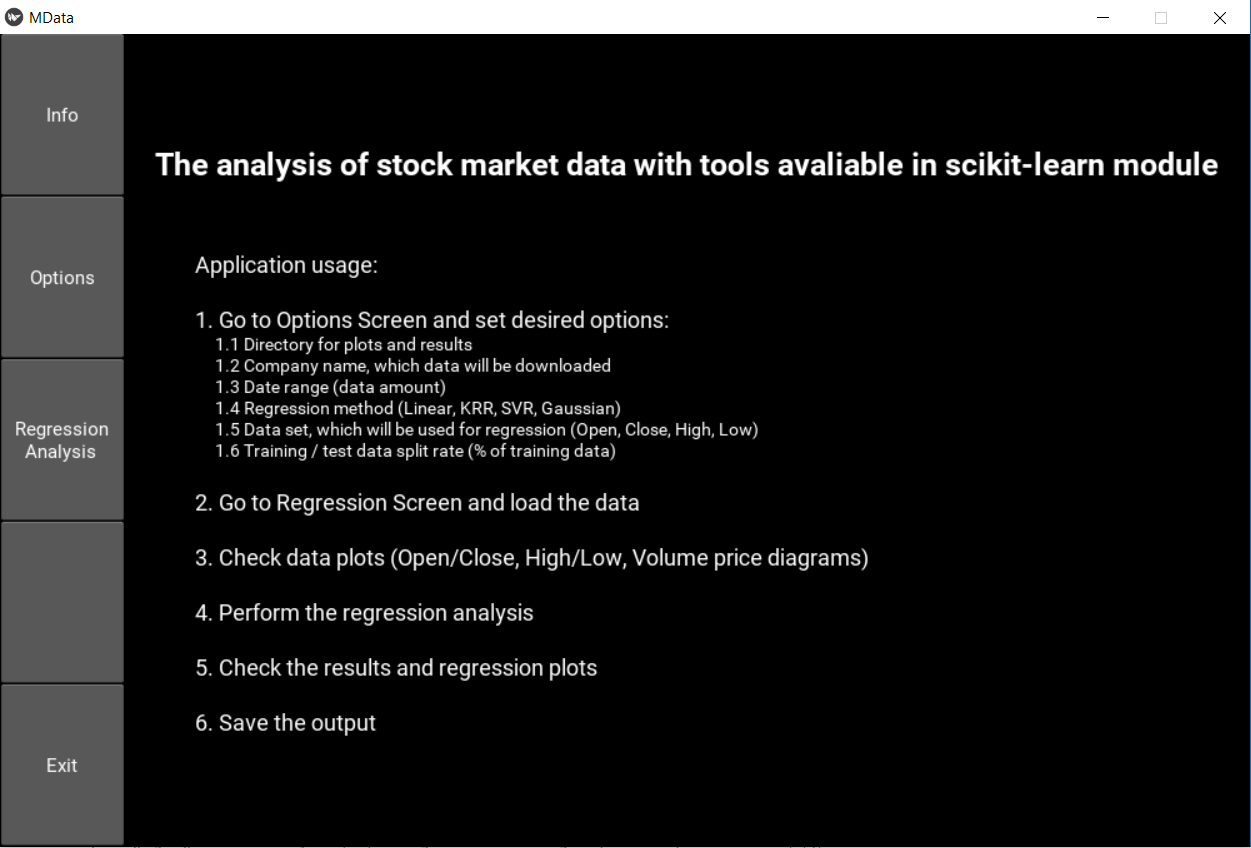
\includegraphics[width=150mm]{pictures/app_info_screen.png}
\caption{Aplikacja: okno instrukcji}
\label{fig:Okno instrukcji}
\end{figure}

Z lewej strony dostępny jest pasek menu, który zawiera przyciski: \textit{Info}, \textit{Options}, \textit{Regression analysis} oraz \textit{Exit}.
Każdy z nich pozwala na wyświetlenie innego okna aplikacji, z wyjątkiem przycisku \textit{Exit} który wywołuje okno z zapytaniem o zakończenie pracy programu.

\subsection{Okno opcji}
W oknie opcji użytkownik może zmienić lub ustawić parametry, które będą używane w późniejszej analizie regresji.
\begin{figure}[h!]
\centering
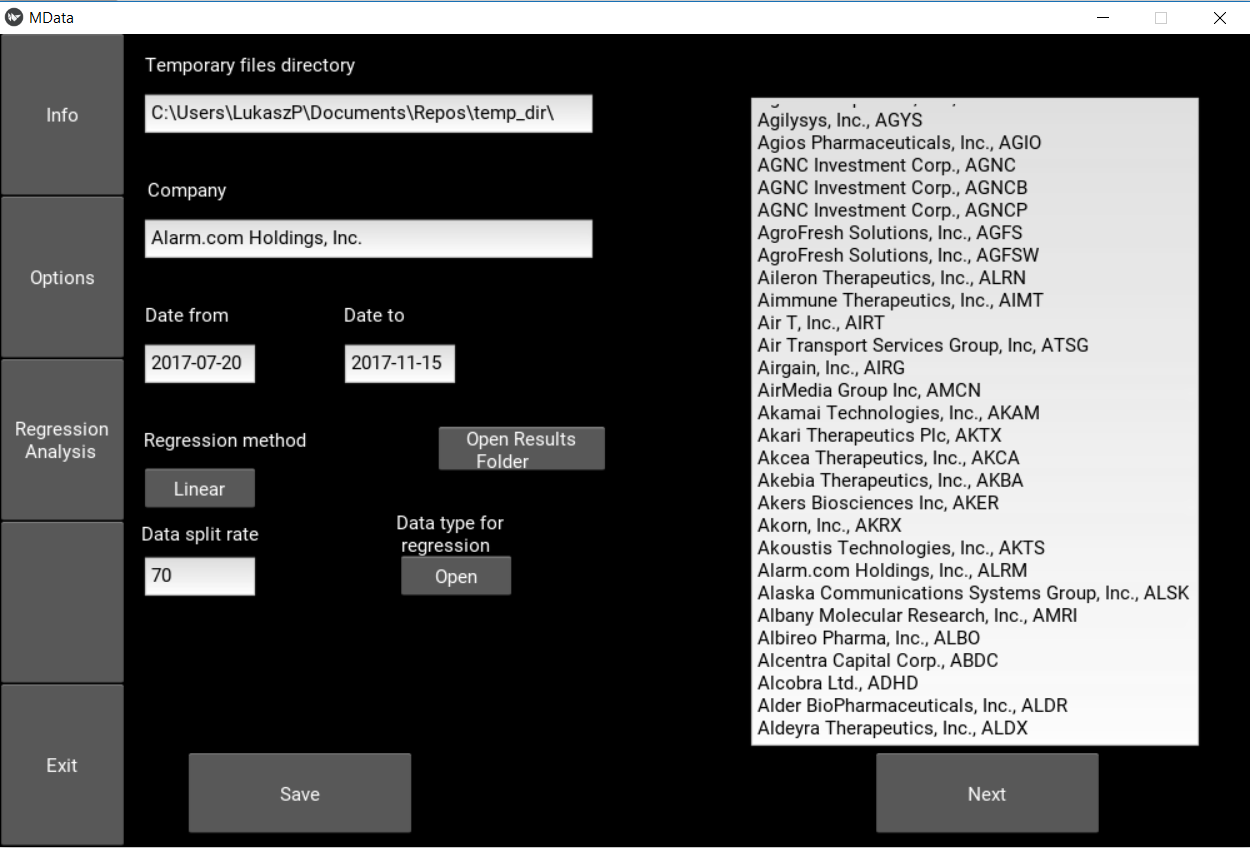
\includegraphics[width=150mm]{pictures/app_options_screen.png}
\caption{Aplikacja: okno instrukcji}
\label{fig:Okno instrukcji}
\end{figure}

Parametry możliwe do zmiany to:
\begin{itemize}
 \item \textit{Temporary files directory}: ścieżka do folderu, do którego mają być zapisywane wyniki
 \item \textit{Company}: nazwa firmy, dla której mają być pobrane dane
 \item \textit{Date from}: data od której mają być pobrane dane, w formacie yyyy-mm-dd
 \item \textit{Date to}: data do której mają być pobierane dane, w formacie yyyy-mm-dd
 \item \textit{Regression method}: lista typu dropdown z możliwością wyboru metody regresji
 \item \textit{Data split rate}: wartość procentowa ilości danych uczących względem danych testowych
 \item \textit{Data type for regression}: lista typu dropdown umożliwiająca wybór typu danych do analizy
\end{itemize}

Do zapisania konfiguracji służy przycisk \textit{Save} który, ze względu na walidację każdego pola lub listy, po wciśnięciu poinformuje użytkownika o powodzeniu lub niepowodzeniu operacji.
W przypadku niepowodzenia użytkownikowi zostaje wskazane pole, które zostało źle wypełnione.\\

Lista firm, dla których jest możliwość pobrania danych znajduje się w zablokowanym polu tekstowym z prawej strony okna.
Jako, iż istnieje możliwość kopiowania tekstu z tego pola, aby wypełnić paramter \textit{Company} należy skopiować dokładną nazwę firmy i wkleić ją we właściwe miejsce.
Przycisk \textit{Next} pozwala natomiast na wyświetlenie kolejnej części listy firm, która jest posortowana alfabetycznie.


\subsection{Okno analizy regresji}

\section{diagramy UML}

%% ------- ROZDZIAŁ 4 ------- %%

\chapter{Testy aplikacji}

\section{Cel przeprowadzonych analiz}

Wykorzystując napisaną na potrzeby niniejszej pracy aplikację przeprowadzono testy, które zmierzają do porównania wybranych modeli regresji dostępnych w pakiecie \textit{Scikit-learn}.\\

Testy przeprowadzone zostały na dwóch zbiorach danych: cen giełdowych firmy Microsoft w zakresie od 2017-01-01 do 2017-10-30, oraz cen giełdowych firmy Intel w zakresie od 2017-01-01 do 2017-04-30.
W dalszej części zbiory te będą nazywane odpowiednio: zbiór szeroki i zbiór wąski.
Dane wykorzystane do testów były cenami otwarcia.\\

Każdy przeprowadzony test uwzględnia wyliczenie dwóch wartości: średniego błędu kwadratowego oraz wyniku predykcji.\\

Średni błąd kwadratowy liczony jest poprzez wykorzystanie funkcji \textit{sklearn.metrics.mean\_squared\_error} z pakietu \textit{Scikit-learn}, a jego wartość w wypadku predykcji idealnej wynosi zero.
Liczony jest na podstawie wartości predykcji dla danych testowych.
Wynik predykcji jest natomiast liczony poprzez wywołanie metody \textit{score()} obieku danego modelu regresji, a jego wartość zmierza do osiągnięcia 1.0 w przypadku idealnym.
Liczony jest na podstawie wyników predykcji zarówno dla zbioru uczącego jak i testowego.\\

Przeprowadzono osobne testy dla każdej z trzech wartości procentowych ilości danych uczących w stosunku do ilości danych testowych: 20\%, 50\% oraz 80\%.\\

Wybrane modele regresji to:
\begin{itemize}
 \item Regresja Liniowa
 \item Regresja Grzbietowa (KRR)
 \item Regresja Wektorów Nośnych (SVR)
 \item Regresja Procesu Gaussa (GPR)
\end{itemize}

Reasumując, dla każdej z metod regresji wykonano sześć testów.\\

Celem testów jest porównanie modeli regresji dostępnych w pakiecie \textit{Scikit-learn} i wyciągnięcie wniosków dotyczących:
\begin{itemize}
 \item dokładności predykcji modeli w zależności od ilości danych uczących oraz całkowitej ilości danych
 \item zdolności modeli do reprezentacji trendu
 \item wpływu zmiany ilości danych uczących na dopasowanie modeli
 \item wpływu całkowitej ilości danych na dopasowanie modeli
\end{itemize}



\section{Testy zbioru danych: Microsoft}

\subsection{Informacje ogólne}
Zakres danych użytych do testów wynosi 209 próbek, w przedziale dat od 2017-01-01 do 2017-10-30 z krokiem wynoszącym jeden dzień.\\

\begin{figure}[h!]
\centering
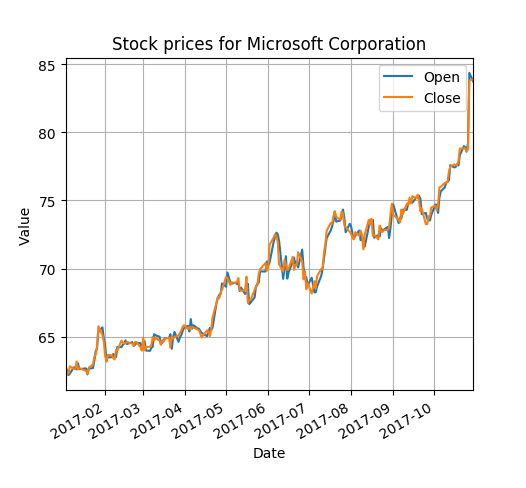
\includegraphics[width=150mm]{pictures/plots/microsoft_oc_price.png}
\caption{Wykres cen otwarcia i zamknięcia firmy Microsoft}
\label{fig:microsoft_oc_price}
\end{figure}

Na rysunku \ref{fig:microsoft_oc_price} przedstawiono wykres zmian cen otwarcia i zamknięcia dla podanego zakresu dat.\\ 

Ilość próbek danych uczących i testowych wynosi odpowiednio:
\begin{itemize}
 \item 41/168 dla wartości 20\% danych uczących
 \item 104/105 dla wartości 50\% danych uczących
 \item 167/42 dla wartości 80\% danych uczących
\end{itemize}
Na przedstawionych wykresach zaznaczona została linia podziału danych uczących i testowych i jest ona reprezentowana przez czerwoną pionową prostą.

\subsection{Regresja liniowa}
Wykres regresji liniowej dla podanego zbioru danych, przy proporcji 20\% danych uczących przedstawiony jest na rysunku \ref{fig:microsoft_linear_20}.\\

\begin{figure}[h!]
\centering
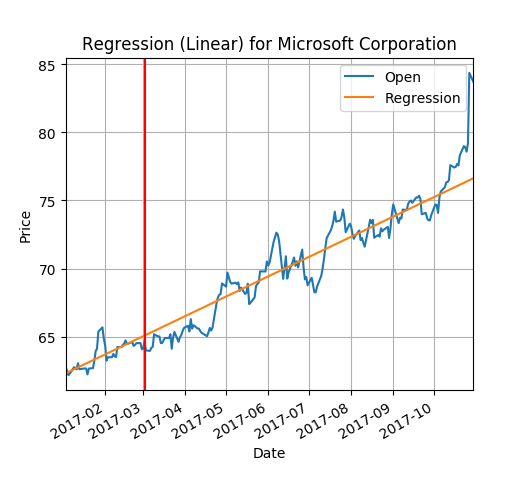
\includegraphics[width=150mm]{pictures/plots/microsoft_linear_20.png}
\caption{Wykres regresji liniowej dla 20\% danych uczących, Microsoft}
\label{fig:microsoft_linear_20}
\end{figure}

Widoczny jest tu trend wzrostowy, który określony na podstawie danych uczących, kontynuowany jest także dla danych testowych.
Należy jednak zauważyć, że podany zbiór danych nie zawiera gwałtownych wzrostów i spadków cen w szczególności w części testowej, dzięki czemu regresja z powodzeniem przewiduje jego kontynuację.\\

Na rysunku \ref{fig:microsoft_linear_50} przedstawiono wykres regresji liniowej dla 50\% proporcji danych uczących.
\begin{figure}[h!]
\centering
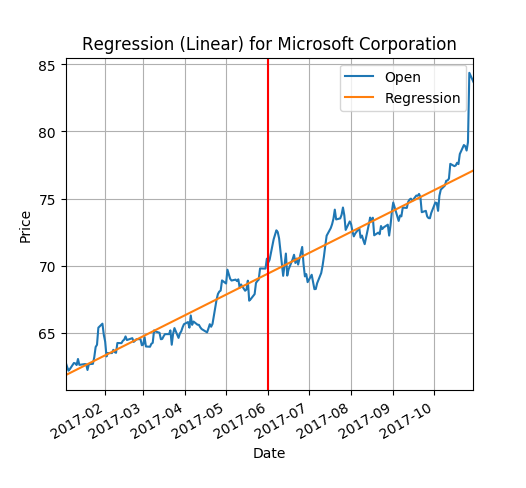
\includegraphics[width=150mm]{pictures/plots/microsoft_linear_50.png}
\caption{Wykres regresji liniowej dla 50\% danych uczących, Microsoft}
\label{fig:microsoft_linear_50}
\end{figure}

Porównując wykresy \ref{fig:microsoft_linear_20} oraz \ref{fig:microsoft_linear_50} zauważalne jest niewielkie przesunięcie prostej regresji w kierunku niższej ceny, 
choć mimo tego można stwierdzić, że dla danego zbioru danych zwiększenie wartości podziału danych na testowe i uczące nie miało wpływu na wynik.

Rysunek \ref{fig:microsoft_linear_80} przedstawia wykres regresji liniowej dla 80\% proporcji danych uczących.\\

\begin{figure}[h!]
\centering
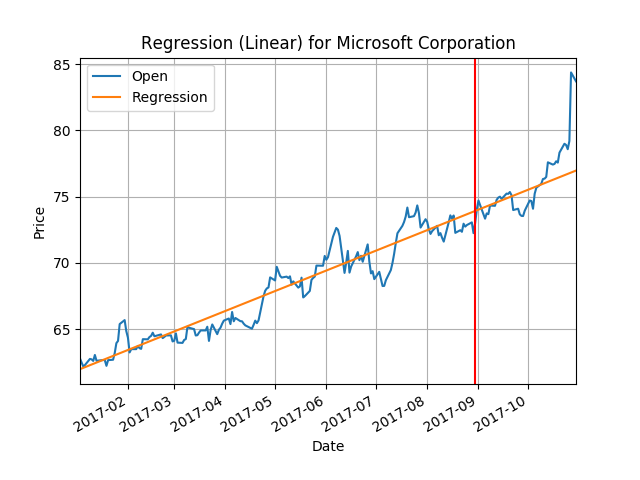
\includegraphics[width=150mm]{pictures/plots/microsoft_linear_80.png}
\caption{Wykres regresji liniowej dla 80\% danych uczących, Microsoft}
\label{fig:microsoft_linear_80}
\end{figure}

W porównaniu do regresji liniowej przeprowadzonej dla 20\% i 50\% danych uczących, wyniki regresji przeprowadzonej dla 80\% danych uczących nie różnią się wiele od pozostałych.
Zauważalne jest jedynie delikatne przesunięcie prostej regresji w kierunku cen niższych, co może być spowodowane przez zmiany kierunku mniejszych trendów obecnych na wykresie.

\subsection{Regresja Grzbietowa}

Rysunki \ref{fig:microsoft_krr_20}, \ref{fig:microsoft_krr_50} i \ref{fig:microsoft_krr_80} przedstawiają wyniki regresji grzbietowej dla 20\%, 50\% i 80\% użytych danych uczących.\\

\begin{figure}[h!]
\centering
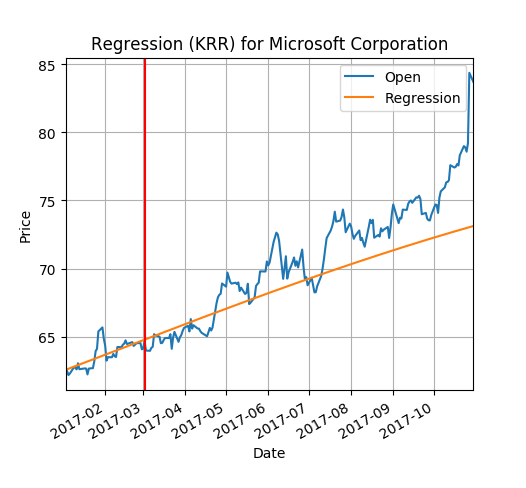
\includegraphics[width=150mm]{pictures/plots/microsoft_krr_20.png}
\caption{Wykres regresji grzbietowej dla 20\% danych uczących, Microsoft}
\label{fig:microsoft_krr_20}
\end{figure}

Krzywa regresji widoczna na powyższym rysunku nie posiada dużych odchyleń, co upodabnia ją do prostej regresji liniowej.
Odchylenie jest zauważalne dopiero przy końcowej części danych testowych. Fakt ten może być spowodowany zbyt małą liczbą danych uczących użytych do przeprowadzenia analizy.\\

\begin{figure}[h!]
\centering
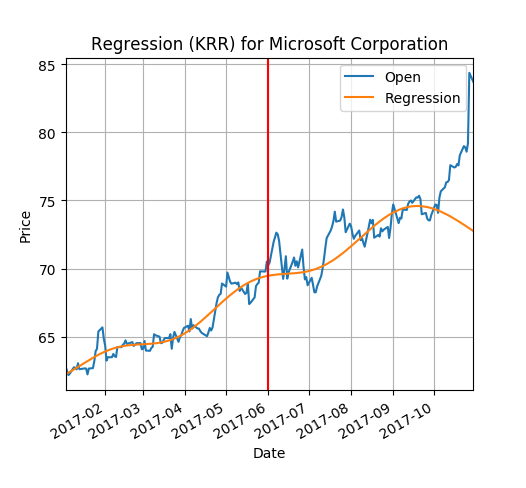
\includegraphics[width=150mm]{pictures/plots/microsoft_krr_50.png}
\caption{Wykres regresji grzbietowej dla 50\% danych uczących, Microsoft}
\label{fig:microsoft_krr_50}
\end{figure}

W porównaniu do rysunku \ref{fig:microsoft_krr_20}, powyższy wykres przedstawia wynik bardziej dokładny i dopasowany.
Zaznaczony jest wyraźny trend wzrostowy z dopasowanymi krzywiznami, które trafnie pokrywają dużą część danych testowych.\\

\begin{figure}[h!]
\centering
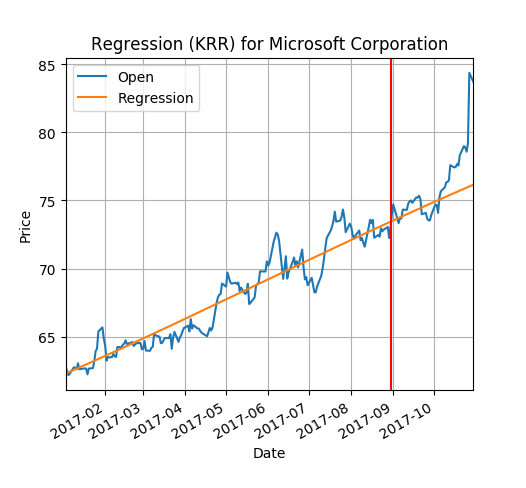
\includegraphics[width=150mm]{pictures/plots/microsoft_krr_80.png}
\caption{Wykres regresji grzbietowej dla 80\% danych uczących, Microsoft}
\label{fig:microsoft_krr_80}
\end{figure}

Wykres przedstawiający wyniki regresji grzbietowej dla największej ilości zastosowanych danych testowych przedstawia krzywą regresji zbliżoną kształtem do prostej.
Może to być spowodowane zastosowaniem zbyt dużej ilości danych uczących, które znajdują się w wyraźnym wzrostowym trendzie o niewielkich odchyleniach.\\

\subsection{Regresja Wektorów Nośnych}

Rysunki \ref{fig:microsoft_svr_20}, \ref{fig:microsoft_svr_50} i \ref{fig:microsoft_svr_80} przedstawiają wykresy wyników regresji wektorów nośnych dla wskazanego zbioru danych, 
o podziale danych uczących względem danych testowych odpowiednio: 20\%, 50\% i 80\%.\\

\begin{figure}[h!]
\centering
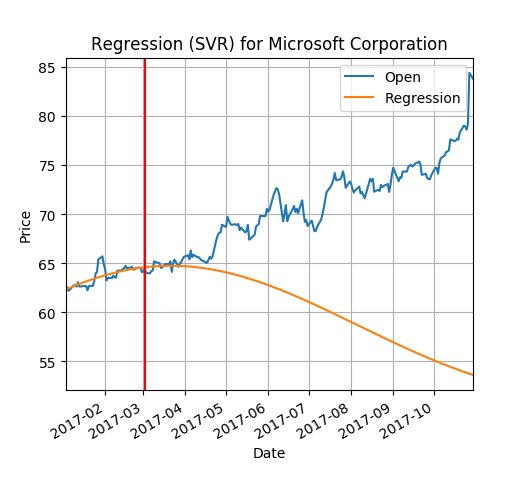
\includegraphics[width=150mm]{pictures/plots/microsoft_svr_20.png}
\caption{Wykres regresji wektorów nośnych dla 20\% danych uczących, Microsoft}
\label{fig:microsoft_svr_20}
\end{figure}

W powyższym przypadku regresja wektorów nośnych wykazuje bardzo niewielkie zdolności predykcyjne, a także niewielkie dopasowanie modelu.
Krzywa regresji po osiągnięciu granicy danych uczących, znacząco odchyla się w kierunku dolnym, coraz bardziej zwiększając błąd predykcji.\\

\begin{figure}[h!]
\centering
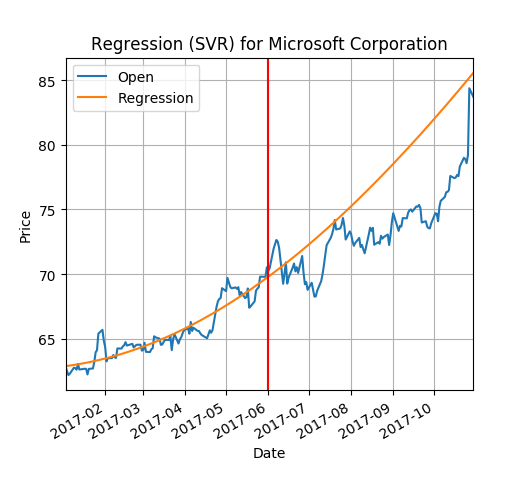
\includegraphics[width=150mm]{pictures/plots/microsoft_svr_50.png}
\caption{Wykres regresji wektorów nośnych dla 50\% danych uczących, Microsoft}
\label{fig:microsoft_svr_50}
\end{figure}

W odróżnieniu od krzywej regresji na rysunku \ref{fig:microsoft_svr_20}, w powyższym przypadku krzywa ta poprawnie przewiduje trend wzrostowy.
Jednakże odchylenie krzywej w stronę górną jest tak silne, że wraz ze wzrostem wartości na osi X wykresu, spada dopasowanie danych.\\

\begin{figure}[h!]
\centering
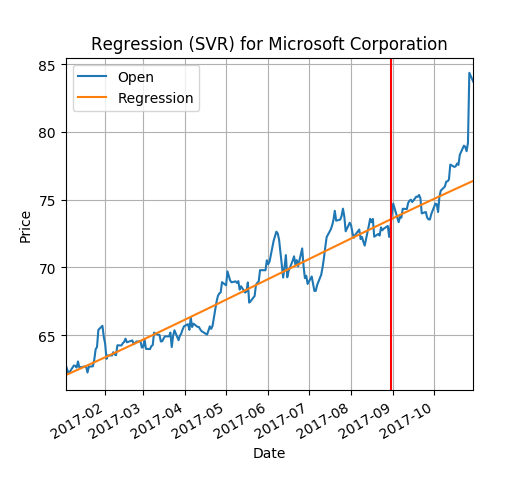
\includegraphics[width=150mm]{pictures/plots/microsoft_svr_80.png}
\caption{Wykres regresji wektorów nośnych dla 80\% danych uczących, Microsoft}
\label{fig:microsoft_svr_80}
\end{figure}

Na wykresie \ref{fig:microsoft_svr_80} można zaobserwować krzywą regresji wektorów nośnych, która przyjmuje postać prostej.
Zachowanie to jest zbieżne z zaobserwowanym na wykresach regresji grzbietowej, co może prowadzić do umocnienia wniosku o użytej zbyt dużej ilości danych uczących przy fakcie, iż dane te reprezentują silny trend wzrostowy.\\

\subsection{Regresja Procesu Gaussa}

Rysunki \ref{fig:microsoft_gpr_20}, \ref{fig:microsoft_gpr_50}, \ref{fig:microsoft_gpr_80} przedstawiają wykresy wyników analiz regresji procesu Gaussa dla odpowiednio: 20\%, 50\% i 80\% zastosowanych danych uczących.\\

\begin{figure}[h!]
\centering
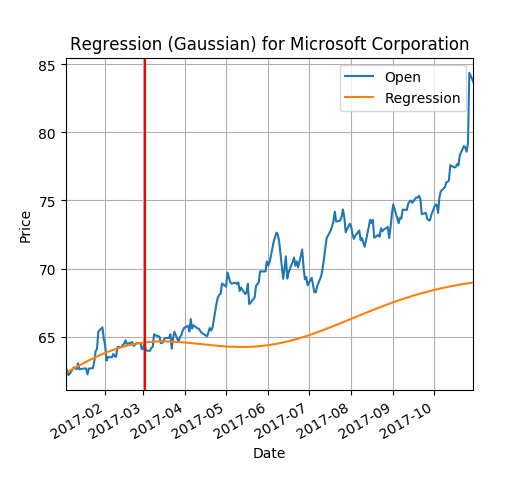
\includegraphics[width=150mm]{pictures/plots/microsoft_gpr_20.png}
\caption{Wykres regresji procesu Gaussa dla 20\% danych uczących, Microsoft}
\label{fig:microsoft_gpr_20}
\end{figure}

Na powyższym wykresie możemy zaobserwować zachowanie się krzywej regresji, które jest bardzo podobne do tej z rysunku \ref{fig:microsoft_svr_20}.
Spowodowane to może być zbyt małą ilością użytych danych uczących, które charakteryzują się niewielką zmiennością.\\

\begin{figure}[h!]
\centering
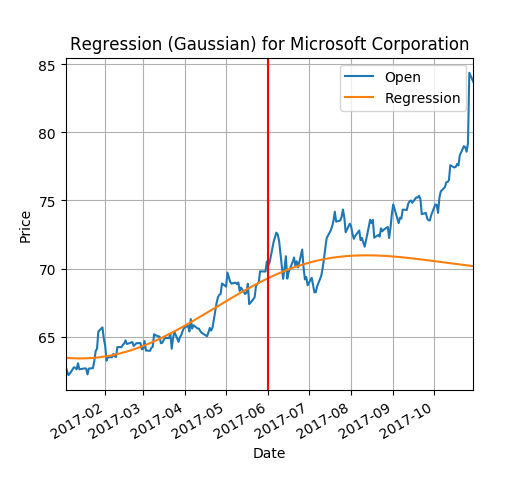
\includegraphics[width=150mm]{pictures/plots/microsoft_gpr_50.png}
\caption{Wykres regresji procesu Gaussa dla 50\% danych uczących, Microsoft}
\label{fig:microsoft_gpr_50}
\end{figure}

Wykres na rysunku \ref{fig:microsoft_gpr_50} powtarza tendencję z wykresu na rysunku \ref{fig:microsoft_gpr_20}.
Trend wzrostowy jest poprawnie przewidywany jedynie dla początkowych wartości danych testowych, a następnie występuje odchylenie krzywej regresji w dół.\\

\begin{figure}[h!]
\centering
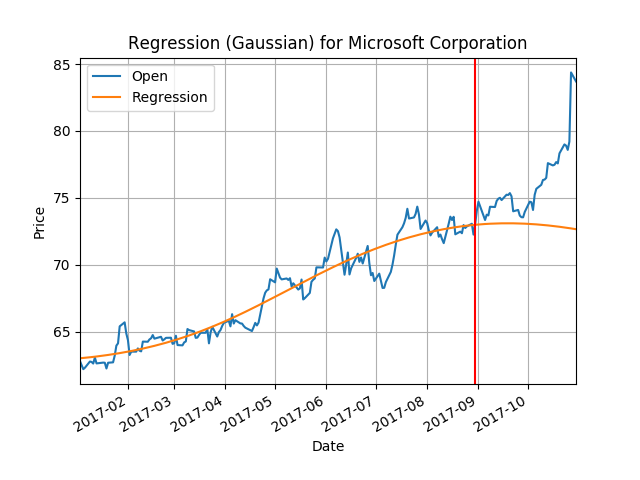
\includegraphics[width=150mm]{pictures/plots/microsoft_gpr_80.png}
\caption{Wykres regresji procesu Gaussa dla 80\% danych uczących, Microsoft}
\label{fig:microsoft_gpr_80}
\end{figure}

Krzywa regresji na powyższym wykresie w odróżnieniu od pozostałych nieliniowych metod regresji, nie wykazuje tendencji do zbliżania się kształtem do prostej.
Jednak predykcja dla zbioru testowego, oraz trend jaki wskazuje krzywa, gorzej odzwierciedlają rzeczywiste dane.\\

\subsection{Podsumowanie}

Podczas dokonanych analiz zebrano dane odnośnie wartości średniego błędu kwadratowego każdej z nich, a także wyniku predykcji. Przedstawiono je na wykresach znajdujących się na rysunkach \ref{fig:microsoft_mean_square} i \ref{fig:microsoft_score}.\\

\begin{figure}[h!]
\centering
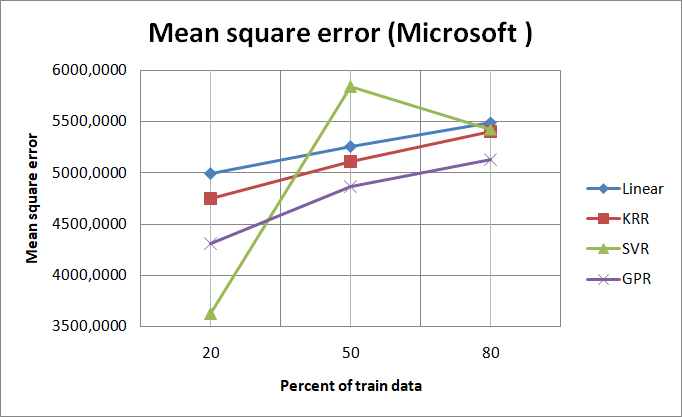
\includegraphics[width=150mm]{pictures/plots/microsoft_mean_square.png}
\caption{Wykres zmian wartości średniego błędu kwadratowego, Microsoft}
\label{fig:microsoft_mean_square}
\end{figure}

\begin{figure}[h!]
\centering
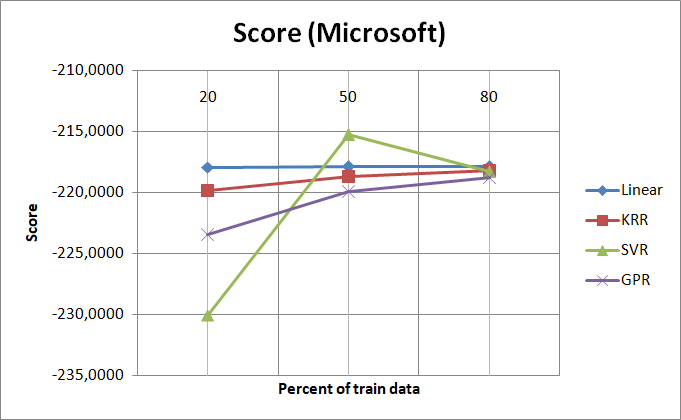
\includegraphics[width=150mm]{pictures/plots/microsoft_score.png}
\caption{Wykres zmian wartości wyników dopasowania modelu, Microsoft}
\label{fig:microsoft_score}
\end{figure}

Z powyższych wykresów wynika, iż średni błąd kwadratowy rośnie wraz ze wzrostem ilości danych uczących zastosowanych w analizie.
Wynik predycji natomiast odznacza się niewielkim wzrostem wraz ze zwiększaną ilością danych uczących.\\

Dla 20\% zastosowanych danych uczących najmniejszy błąd osiągnęła regresja wektorów nośnych, zaś największy - liniowa.
W przypadku wyniku predykcji jest natomiast odwrotnie: najlepszą wartość osiągnęła regresja liniowa,  a najgorszą regresja wektorów nośnych.\\

Dla 50\% zastosowanych danych uczących najmniejszym błędem kwadratowym charakteryzuje się regresja procesu Gaussa, a najwyższym regresja wektorów nośnych.
Powtórzona zostaje zależność zidentyfikowana w przypadku 20\% danych uczących: wynik predykcji oceniany najlepiej należy do regresji wektorów nośnych, natomiast najgorzej do regrtesji procesu Gaussa\\

W przypadku 80\% zastosowanych danych testowych regresja procesu Gaussa osiągnęła najniższy wynik średniego błędu kwadratowego. Pozostałe modele regresji charakteryzują się zbliżonym wynikiem.
Wynik predykcji dla każdego z modeli jest w tym przypadku bardzo zbliżony.\\

Na podstawie zgromadzonych wykresów, a także powyższych danych, można określić następujące wnioski:
\begin{itemize}
 \item trafne określenie trendu dla danych testowych zaobserwowano w przypadkach regresji liniowej, wektorów nośnych (80\% danych uczących) oraz grzbietowej (20\% i 80\% danych uczących)
 \item krzywe regresji, które nie identyfikowały poprawnie trendu dla danych testowych należą do regresji wektorów nośnych (20\% danych testowych) oraz procesu Gaussa
 \item w przypadku regresji grzbietowej (50\% danych uczących), zaobserwowano dobre dopasowanie i potwierdzenie trendu dla około 80\% danych testowych, po czym następowała zmiana nachylenia krzywej
\end{itemize}


\section{Testy zbioru danych: Intel}

\subsection{Informacje ogólne}
Zakres danych użytych do testów wynosi 81 próbek, w przedziale dat od 2017-01-01 do 2017-14-30 z krokiem wynoszącym jeden dzień.\\
Zakres ten charakteryzuje się mniejszą ilością danych o większej zmienności, niż zakres poprzedni.

\begin{figure}[h!]
\centering
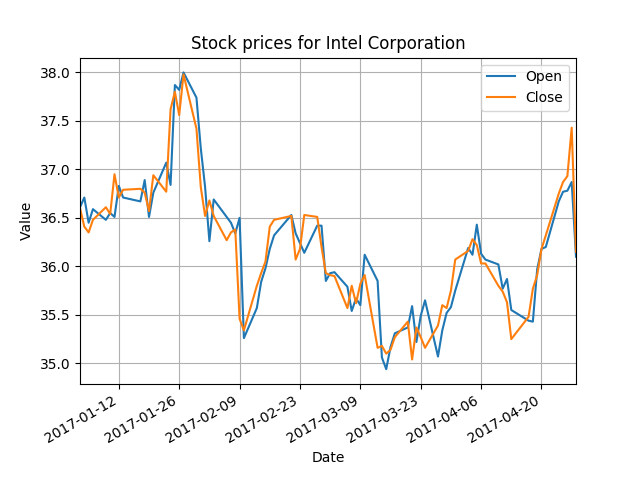
\includegraphics[width=150mm]{pictures/plots/intel_oc_price.png}
\caption{Wykres cen otwarcia i zamknięcia firmy Intel}
\label{fig:intel_oc_price}
\end{figure}

Na rysunku \ref{fig:intel_oc_price} przedstawiono wykres zmian cen otwarcia i zamknięcia dla podanego zakresu dat.\\ 

Ilość próbek danych uczących i testowych wynosi odpowiednio:
\begin{itemize}
 \item 16/65 dla wartości 20\% danych uczących
 \item 40/41 dla wartości 50\% danych uczących
 \item 64/17 dla wartości 80\% danych uczących
\end{itemize}

\subsection{Regresja liniowa}

Na wykresach \ref{fig:intel_linear_20}, \ref{fig:intel_linear_50} oraz \ref{fig:intel_linear_80} przedstawiono wyniko regresji liniowej o udziale danych uczących odpowiednio: 20\%, 50\% i 80\%.\\

\begin{figure}[h!]
\centering
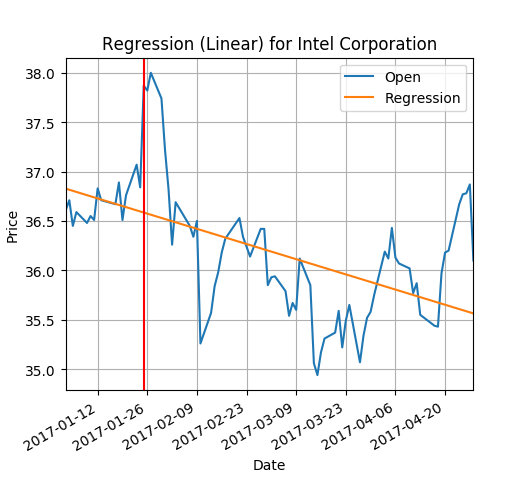
\includegraphics[width=150mm]{pictures/plots/intel_linear_20.png}
\caption{Wykres regresji liniowej dla 20\% danych uczących, Intel}
\label{fig:intel_linear_20}
\end{figure}

Z powyższego wykresu wynika, iż poprzez predykcję poprawnie zidentyfikowano trend spadkowy.\\

\begin{figure}[h!]
\centering
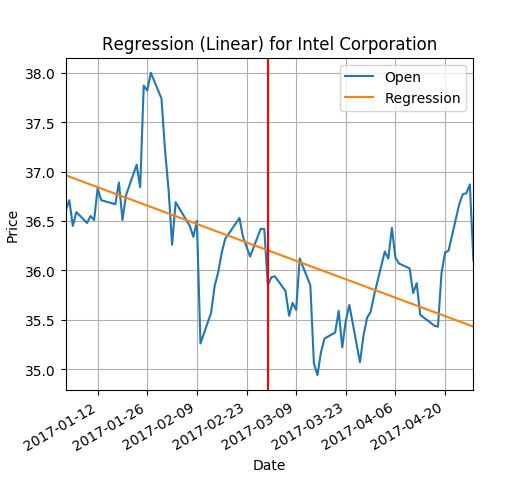
\includegraphics[width=150mm]{pictures/plots/intel_linear_50.png}
\caption{Wykres regresji liniowej dla 50\% danych uczących, Intel}
\label{fig:intel_linear_50}
\end{figure}

W porównaniu do wykresu na rysunku \ref{fig:intel_linear_50}, na powyższym wykresie zaobserwować można prostą regresji identyfikującą trend spadkowy, lecz o mniejszym nachyleniu niż poprzednio.
Może być to spowodowane lepszym dopasowaniem modelu, lub też zwiększoną liczbą danych uczących.\\

\begin{figure}[h!]
\centering
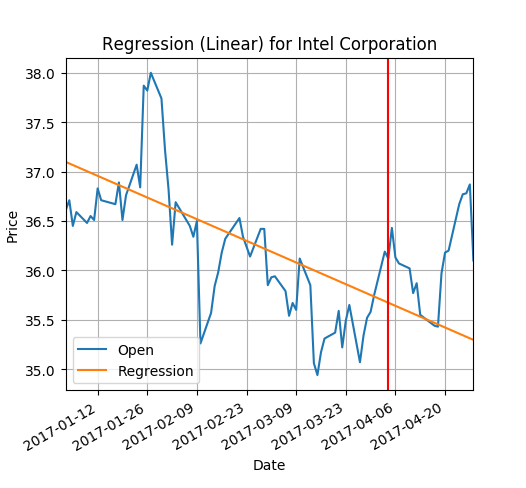
\includegraphics[width=150mm]{pictures/plots/intel_linear_80.png}
\caption{Wykres regresji liniowej dla 80\% danych uczących, Intel}
\label{fig:intel_linear_80}
\end{figure}

Porównując wszystkie trzy powyższe analizy regresji liniowej, można zaobserwować zależność spadku nachylenia prostej regresji od ilości zastosowanych danych uczących.

\subsection{Regresja Grzbietowa}

Na rysunkach \ref{fig:intel_krr_20}, \ref{fig:intel_krr_50} i \ref{fig:intel_krr_80} przedstawiono wyniko analizy regresji grzbietowej, przy zastosowaniu 20\%, 50\% i 80\% danych uczących.\\

\begin{figure}[h!]
\centering
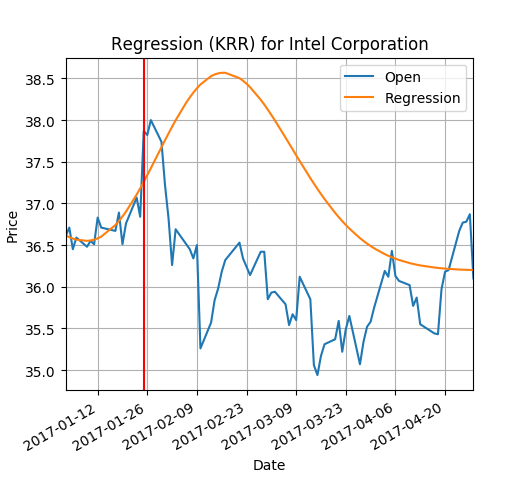
\includegraphics[width=150mm]{pictures/plots/intel_krr_20.png}
\caption{Wykres regresji grzbietowej dla 20\% danych uczących, Intel}
\label{fig:intel_krr_20}
\end{figure}

Powyższy wykres wykazuje błędną predykcję i rozpoznanie trendu, które mogą być skutkiem zbyt małej ilości danych uczących.
Poza tym, dane zakres danych testowych obejmuje jedynie mniejszy trend wzrostowy, przez co utrudniona lub niemożliwa jest identyfikacja szerszego trendu spadkowego.\\

\begin{figure}[h!]
\centering
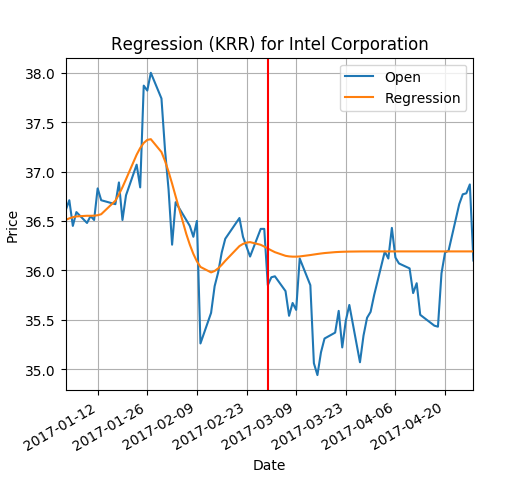
\includegraphics[width=150mm]{pictures/plots/intel_krr_50.png}
\caption{Wykres regresji grzbietowej dla 50\% danych uczących, Intel}
\label{fig:intel_krr_50}
\end{figure}

Wykres \ref{fig:intel_krr_50} przedstawia krzywą regresji, która charakteryzuje się dobrym dopasowaniem w części danych uczących, lecz w części danych testowych staje się ona niemal linią prostą.
Może być to ponownie spowodowane nietrafnie dobranym zakresem danych uczących, ponieważ można w nim zaobserwować zarówno duży wzrost i duży spadek, co w połączeniu z małą ilością próbek danych może czynić zbiór niereprezentacyjnym.\\

\begin{figure}[h!]
\centering
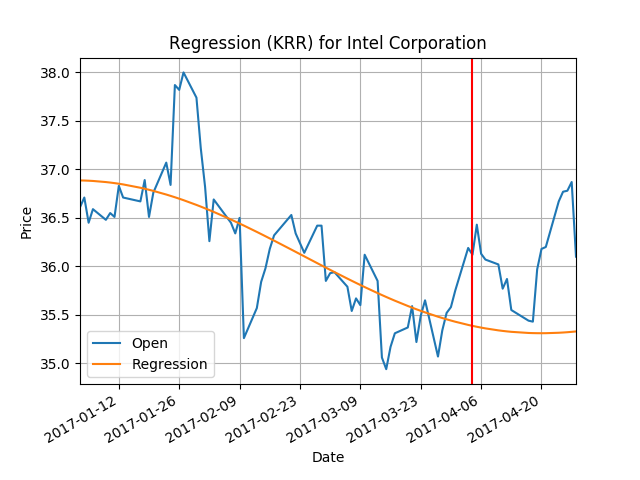
\includegraphics[width=150mm]{pictures/plots/intel_krr_80.png}
\caption{Wykres regresji grzbietowej dla 80\% danych uczących, Intel}
\label{fig:intel_krr_80}
\end{figure}

Spośród trzech przedstawionych analiz regresji grzbietowej, wykres na rysunku \ref{fig:intel_krr_80} zdecydowanie przedstawia krzywą regresji najlepiej przedstawiającą trend.
Należy jednak zauważyć, iż fragment przedstawiający dane testowe jest relatywnie niewielki, a przewidywane wartości nie pokrywają się w żadnym punkcie z wartościami testowymi.\\

\subsection{Regresja Wektorów Nośnych}

Rysunki \ref{fig:intel_svr_20}, \ref{fig:intel_svr_50} i \ref{fig:intel_svr_80} przedstawiają wykresy analizy regresji wektorów nośnych dla proporcji danych uczących wynoszących odpowiednio: 20\%, 50\% i 80\%.\\

\begin{figure}[h!]
\centering
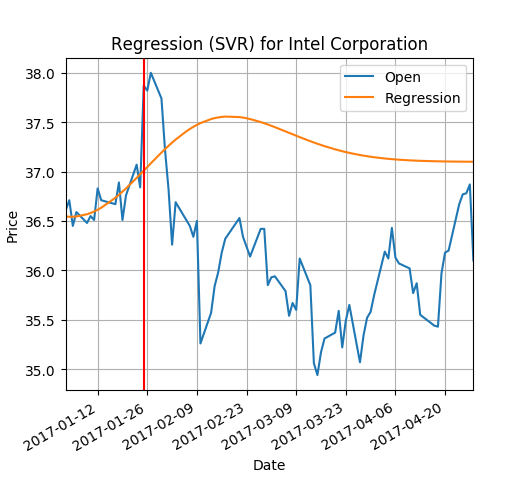
\includegraphics[width=150mm]{pictures/plots/intel_svr_20.png}
\caption{Wykres regresji wektorów nośnych dla 20\% danych uczących, Intel}
\label{fig:intel_svr_20}
\end{figure}

Powyższy wykres przedstawia podobną zależność, co wykres analizy regresji grzbietowej dla tych samych ilości danych uczących.
Podtrzymany zostaje więc wniosek, iż niepoprawna identyfikacja trendu spowodowana może być złym dobraniem danych uczących, reprezentujących jedynie mniejszy trend wzrostowy.\\

\begin{figure}[h!]
\centering
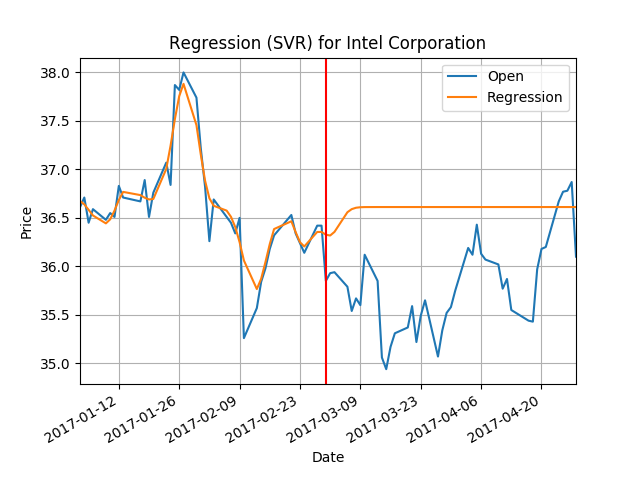
\includegraphics[width=150mm]{pictures/plots/intel_svr_50.png}
\caption{Wykres regresji wektorów nośnych dla 50\% danych uczących, Intel}
\label{fig:intel_svr_50}
\end{figure}

Wykres na rysunku \ref{fig:intel_svr_50} wykazuje poprawne dopasowanie modelu regresji w części danych uczących, lecz w części danych testowych błędnie identyfikuje trend, a krzywa regresji przybiera postać prostej.
Może to być spowodowane błędnym dobraniem parametrów obiektu \textit{SVR()}.\\

\begin{figure}[h!]
\centering
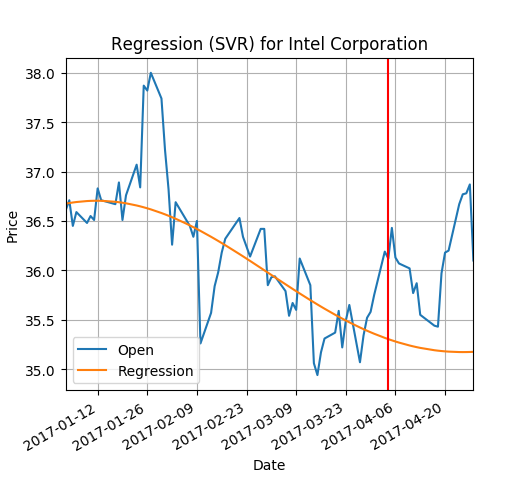
\includegraphics[width=150mm]{pictures/plots/intel_svr_80.png}
\caption{Wykres regresji wektorów nośnych dla 80\% danych uczących, Intel}
\label{fig:intel_svr_80}
\end{figure}

Podobnie jak w przypadku wykresu \ref{fig:intel_krr_80} regresji grzbietowej, także i w powyższym przypadku dopasowanie modelu i identyfikacja trendu spadkowego są zauważalne.\\

\subsection{Regresja Procesu Gaussa}

Na rysunkach \ref{fig:intel_gpr_20}, \ref{fig:intel_gpr_50} i \ref{fig:intel_gpr_80} przedstawiono wykresy analizy regresji procesu Gaussa dla następujących ilości danych testowych: 20\%, 50\% i 80\%.\\

\begin{figure}[h!]
\centering
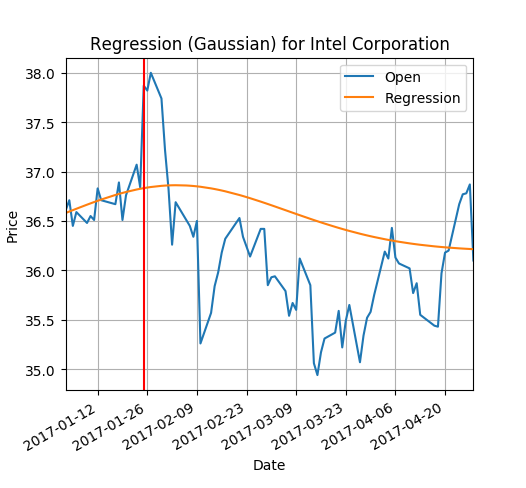
\includegraphics[width=150mm]{pictures/plots/intel_gpr_20.png}
\caption{Wykres regresji procesu Gaussa dla 20\% danych uczących, Intel}
\label{fig:intel_gpr_20}
\end{figure}

W powyższym przypadku krzywa regresji poprawnie identyfikuje trend spadkowy w części testowej, jednakże niewielkie nachylenie krzywej nie oddaje do końca charakteru spadkowego danych.\\ 

\begin{figure}[h!]
\centering
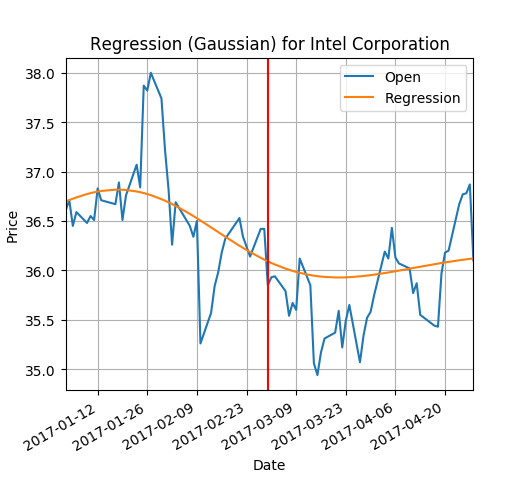
\includegraphics[width=150mm]{pictures/plots/intel_gpr_50.png}
\caption{Wykres regresji procesu Gaussa dla 50\% danych uczących, Intel}
\label{fig:intel_gpr_50}
\end{figure}

Na rysunku \ref{fig:intel_gpr_50} można zaobserwować krzywą regresji poprawnie opisującą i przewidującą przebieg trendu.
W części danych testowych zauważalny jest nie tylko delikatny spadek, lecz również wzrost dla końcowych wartości danych, co zgadza się z wartościami testowymi.\\

\begin{figure}[h!]
\centering
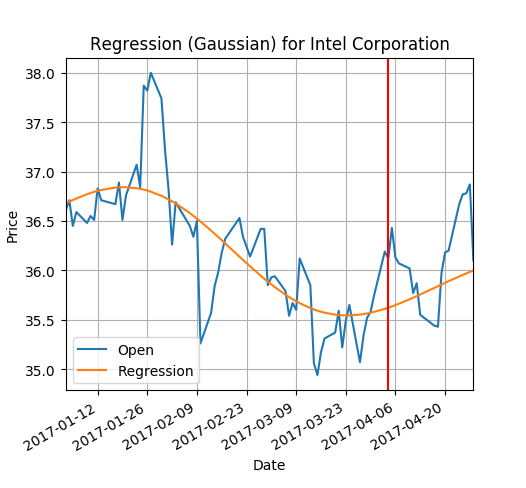
\includegraphics[width=150mm]{pictures/plots/intel_gpr_80.png}
\caption{Wykres regresji procesu Gaussa dla 80\% danych uczących, Intel}
\label{fig:intel_gpr_80}
\end{figure}

W porównaniu do poprzednich wyników regresji procesu Gaussa, powyższy wykres potwierdza wniosek, iż wraz ze wzrostem ilości danych testowych dla tego zbioru danych, rośnie dopasowanie modelu oraz jakość predykcji.\\

\subsection{Podsumowanie}

Dane dotyczące średniego błędu kwadratowego oraz wyników predykcji modeli regresji są przedstawione na wykresach \ref{fig:intel_mean_square} oraz \ref{fig:intel_score}.\\

\begin{figure}[h!]
\centering
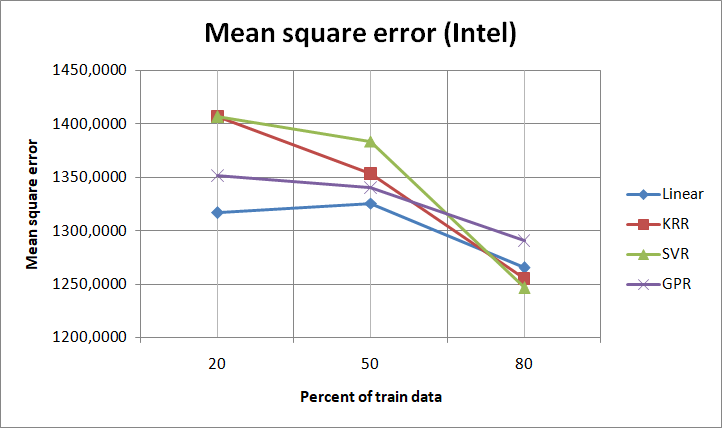
\includegraphics[width=150mm]{pictures/plots/intel_mean_square.png}
\caption{Wykres zmian wartości średniego błędu kwadratowego, Intel}
\label{fig:intel_mean_square}
\end{figure}

\begin{figure}[h!]
\centering
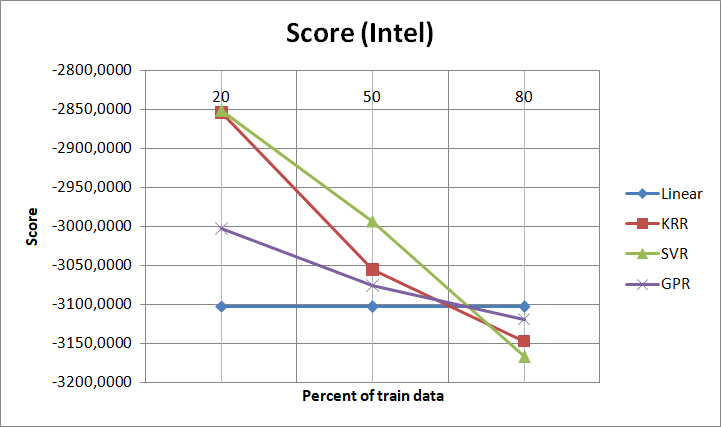
\includegraphics[width=150mm]{pictures/plots/intel_score.png}
\caption{Wykres zmian wartości wyników dopasowania modelu, Intel}
\label{fig:intel_score}
\end{figure}

Z powyższych danych wynika, iż dla ilości danych uczących wynoszącej 20\% najwyższy średni błąd kwadratowy uzyskały modele regresji wektorów nośnych oraz grzbietowa, najniższy zaś model regresji liniowej.
Dla ilości danych uczących wynoszącej 50\% najwyższa wartość błędu odnosi się do modelu regresji wektorów nośnych, a najniższa do modelu regresji liniowej.
Dla 80\% danych uczących natomiast, wszystkie modele regresji osiągnęły podobną, niską wartość, z wyjątkiem modelu regresji procesu Gaussa, który osiągnął wartość najwyższą.\\

W odróżnieniu od poprzedniego testowanego zakresu danych, w tym przypadku zaobserwować można tendencję spadku wartości średniego kwadratu błędów wraz ze wzrostem procentowej ilości użytych danych uczących.\\

Z wykresu \ref{fig:intel_score} wynika, iż wraz ze wzrostem ilości użytych danych uczących spada wartość dopasowania każdego modelu, z wyjątkiem modelu liniowego, który przedstawia za każdym razem podobną wartość.
Może być to spowodowane faktem, iż wartość ta jest liczona jedynie dla danych testowych, więc przy zmniejszaniu ich ilości obserwujemy spadek dopasowania.\\

Analiza wykresów pozwala wnioskować, iż trafne określenie trendu można dostrzec na wykresach regresji procesu Gaussa, liniowej, grzbietowej (80\% danych uczących) oraz wektorów nośnych (80\% danych uczących).
Natomiast niedokładna predykcja trendu widoczna jest na wykresach regresji grzbietowej (20\% i 50\% danych uczących) oraz wektorów nośnych (20\% i 50\% danych uczących).\\

\section{Wnioski}

\begin{enumerate}
 \item Dokładność predykcji modelu regresji liniowej zmienia się nieznacznie w zależności od zmiany proporcji ilości danych uczących względem danych testowych.
 \item Przedstawione modele regresji nieliniowych wykazują dużą wrażliwość na wysoką zmienność danych poddawanych analizie, przez co w celu osiągnięcia bardziej dokładnych wyników predykcji niezbędne jest znalezienie właściwych zakresów parametrów podawanych jako argumenty do obiektów tych regresji.
 \item Wartości średniego kwadratu błędów oraz wyników predykcji (dopasowania modelu) wykazują zależność od całkowitej ilości analizowanych danych. Wraz ze wzrostem ich ilości zwiększają się wartości błędów, a wyniki predykcji ulegają polepszeniu.
 \item Dobre właściwości określania trendu dla obydwu testowanych zakresów danych wykazały: regresja liniowa, wektorów nośnych (przy 80\% danych uczących) oraz grzbietowa (przy 80\% danych uczących).
 \item Regresja procesu Gaussa w przypadku dużego zbioru danych nie wykazała dobrych zdolności predykcyjnych, natomiast w przypadku małego zbioru można ją uznać za najlepszą metodę regresji dla podanych warunków.
 \item Jakość predykcji za pomocą testowanych metod w dużym stopniu zależy od struktury danych użytych do analizy. Jednocześnie najbardziej odporną na ten czynnik metodą okazała się regresja liniowa.
 \item Wraz ze wzrostem ilości użytych do analizy danych uczących, w większości przypadków wzrasta trafność predykcji lub trafność określenia trendu.
 \item Pakiet \textit{Scikit-learn} i udostępniane przez niego metody regresji są przydatne w analizie danych giełdowych. Ich dokładność można zwiększyć odpowiednio parametryzując tworzone obiekty modeli regresji, oraz poprawnie dobierając dane.
\end{enumerate}



%% ------- ROZDZIAŁ 5 ------- %%

\chapter{Wnioski}



%%% ------- ROZDZIAŁ 4 ------- %%

\chapter{Testy aplikacji}

\section{Cel przeprowadzonych analiz}

Wykorzystując napisaną na potrzeby niniejszej pracy aplikację przeprowadzono testy, które zmierzają do porównania wybranych modeli regresji dostępnych w pakiecie \textit{Scikit-learn}.\\

Testy przeprowadzone zostały na dwóch zbiorach danych: cen giełdowych firmy Microsoft w zakresie od 2017-01-01 do 2017-10-30, oraz cen giełdowych firmy Intel w zakresie od 2017-01-01 do 2017-04-30.
W dalszej części zbiory te będą nazywane odpowiednio: zbiór szeroki i zbiór wąski.
Dane wykorzystane do testów były cenami otwarcia.\\

Każdy przeprowadzony test uwzględnia wyliczenie dwóch wartości: średniego błędu kwadratowego oraz wyniku predykcji.\\

Średni błąd kwadratowy liczony jest poprzez wykorzystanie funkcji \textit{sklearn.metrics.mean\_squared\_error} z pakietu \textit{Scikit-learn}, a jego wartość w wypadku predykcji idealnej wynosi zero.
Liczony jest na podstawie wartości predykcji dla danych testowych.
Wynik predykcji jest natomiast liczony poprzez wywołanie metody \textit{score()} obieku danego modelu regresji, a jego wartość zmierza do osiągnięcia 1.0 w przypadku idealnym.
Liczony jest na podstawie wyników predykcji zarówno dla zbioru uczącego jak i testowego.\\

Przeprowadzono osobne testy dla każdej z trzech wartości procentowych ilości danych uczących w stosunku do ilości danych testowych: 20\%, 50\% oraz 80\%.\\

Wybrane modele regresji to:
\begin{itemize}
 \item Regresja Liniowa
 \item Regresja Grzbietowa (KRR)
 \item Regresja Wektorów Nośnych (SVR)
 \item Regresja Procesu Gaussa (GPR)
\end{itemize}

Reasumując, dla każdej z metod regresji wykonano sześć testów.\\

Celem testów jest porównanie modeli regresji dostępnych w pakiecie \textit{Scikit-learn} i wyciągnięcie wniosków dotyczących:
\begin{itemize}
 \item dokładności predykcji modeli w zależności od ilości danych uczących oraz całkowitej ilości danych
 \item zdolności modeli do reprezentacji trendu
 \item wpływu zmiany ilości danych uczących na dopasowanie modeli
 \item wpływu całkowitej ilości danych na dopasowanie modeli
\end{itemize}



\section{Testy zbioru danych: Microsoft}

\subsection{Informacje ogólne}
Zakres danych użytych do testów wynosi 209 próbek, w przedziale dat od 2017-01-01 do 2017-10-30 z krokiem wynoszącym jeden dzień.\\

\begin{figure}[h!]
\centering
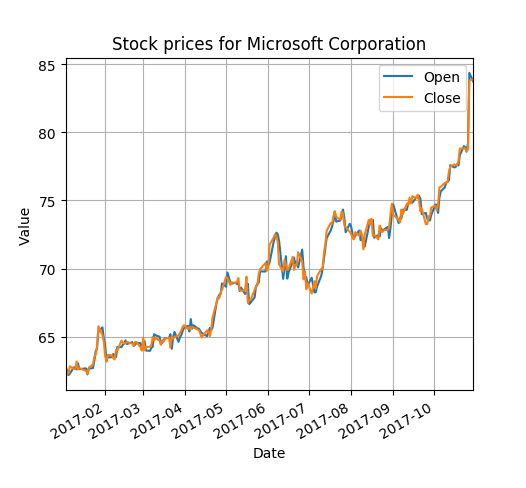
\includegraphics[width=150mm]{pictures/plots/microsoft_oc_price.png}
\caption{Wykres cen otwarcia i zamknięcia firmy Microsoft}
\label{fig:microsoft_oc_price}
\end{figure}

Na rysunku \ref{fig:microsoft_oc_price} przedstawiono wykres zmian cen otwarcia i zamknięcia dla podanego zakresu dat.\\ 

Ilość próbek danych uczących i testowych wynosi odpowiednio:
\begin{itemize}
 \item 41/168 dla wartości 20\% danych uczących
 \item 104/105 dla wartości 50\% danych uczących
 \item 167/42 dla wartości 80\% danych uczących
\end{itemize}
Na przedstawionych wykresach zaznaczona została linia podziału danych uczących i testowych i jest ona reprezentowana przez czerwoną pionową prostą.

\subsection{Regresja liniowa}
Wykres regresji liniowej dla podanego zbioru danych, przy proporcji 20\% danych uczących przedstawiony jest na rysunku \ref{fig:microsoft_linear_20}.\\

\begin{figure}[h!]
\centering
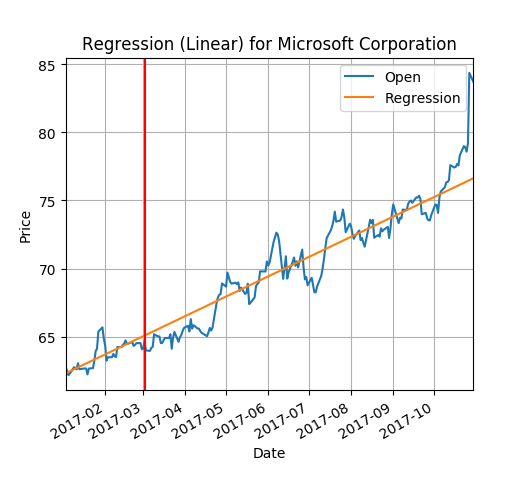
\includegraphics[width=150mm]{pictures/plots/microsoft_linear_20.png}
\caption{Wykres regresji liniowej dla 20\% danych uczących, Microsoft}
\label{fig:microsoft_linear_20}
\end{figure}

Widoczny jest tu trend wzrostowy, który określony na podstawie danych uczących, kontynuowany jest także dla danych testowych.
Należy jednak zauważyć, że podany zbiór danych nie zawiera gwałtownych wzrostów i spadków cen w szczególności w części testowej, dzięki czemu regresja z powodzeniem przewiduje jego kontynuację.\\

Na rysunku \ref{fig:microsoft_linear_50} przedstawiono wykres regresji liniowej dla 50\% proporcji danych uczących.
\begin{figure}[h!]
\centering
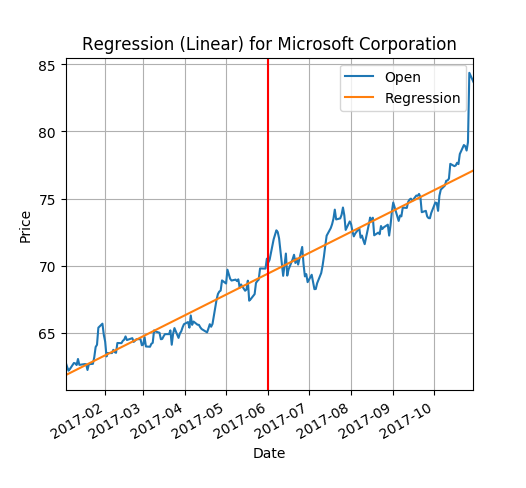
\includegraphics[width=150mm]{pictures/plots/microsoft_linear_50.png}
\caption{Wykres regresji liniowej dla 50\% danych uczących, Microsoft}
\label{fig:microsoft_linear_50}
\end{figure}

Porównując wykresy \ref{fig:microsoft_linear_20} oraz \ref{fig:microsoft_linear_50} zauważalne jest niewielkie przesunięcie prostej regresji w kierunku niższej ceny, 
choć mimo tego można stwierdzić, że dla danego zbioru danych zwiększenie wartości podziału danych na testowe i uczące nie miało wpływu na wynik.

Rysunek \ref{fig:microsoft_linear_80} przedstawia wykres regresji liniowej dla 80\% proporcji danych uczących.\\

\begin{figure}[h!]
\centering
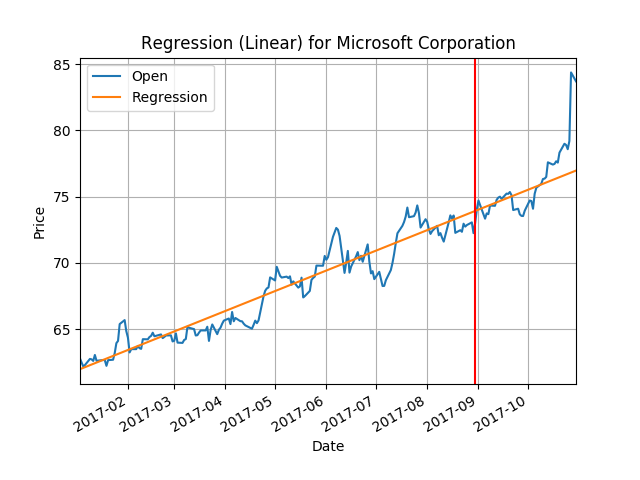
\includegraphics[width=150mm]{pictures/plots/microsoft_linear_80.png}
\caption{Wykres regresji liniowej dla 80\% danych uczących, Microsoft}
\label{fig:microsoft_linear_80}
\end{figure}

W porównaniu do regresji liniowej przeprowadzonej dla 20\% i 50\% danych uczących, wyniki regresji przeprowadzonej dla 80\% danych uczących nie różnią się wiele od pozostałych.
Zauważalne jest jedynie delikatne przesunięcie prostej regresji w kierunku cen niższych, co może być spowodowane przez zmiany kierunku mniejszych trendów obecnych na wykresie.

\subsection{Regresja Grzbietowa}

Rysunki \ref{fig:microsoft_krr_20}, \ref{fig:microsoft_krr_50} i \ref{fig:microsoft_krr_80} przedstawiają wyniki regresji grzbietowej dla 20\%, 50\% i 80\% użytych danych uczących.\\

\begin{figure}[h!]
\centering
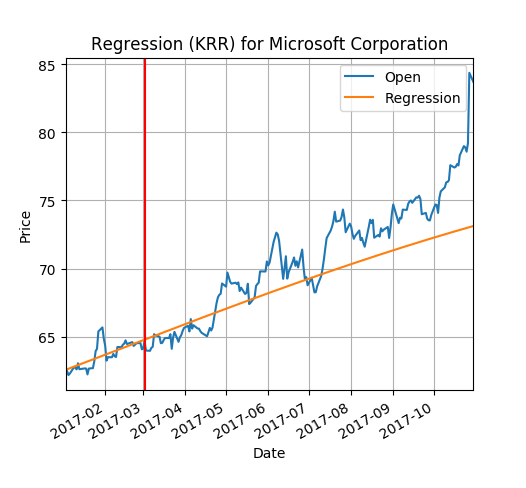
\includegraphics[width=150mm]{pictures/plots/microsoft_krr_20.png}
\caption{Wykres regresji grzbietowej dla 20\% danych uczących, Microsoft}
\label{fig:microsoft_krr_20}
\end{figure}

Krzywa regresji widoczna na powyższym rysunku nie posiada dużych odchyleń, co upodabnia ją do prostej regresji liniowej.
Odchylenie jest zauważalne dopiero przy końcowej części danych testowych. Fakt ten może być spowodowany zbyt małą liczbą danych uczących użytych do przeprowadzenia analizy.\\

\begin{figure}[h!]
\centering
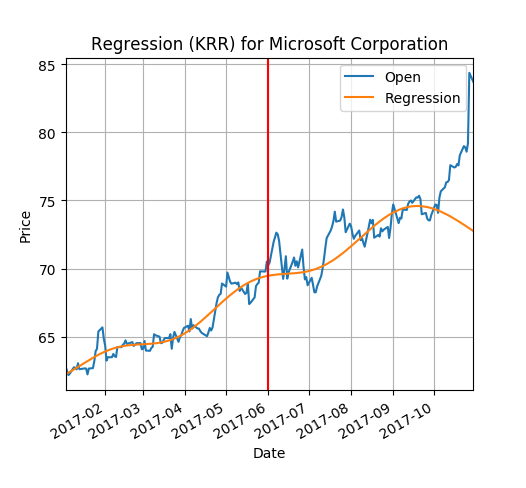
\includegraphics[width=150mm]{pictures/plots/microsoft_krr_50.png}
\caption{Wykres regresji grzbietowej dla 50\% danych uczących, Microsoft}
\label{fig:microsoft_krr_50}
\end{figure}

W porównaniu do rysunku \ref{fig:microsoft_krr_20}, powyższy wykres przedstawia wynik bardziej dokładny i dopasowany.
Zaznaczony jest wyraźny trend wzrostowy z dopasowanymi krzywiznami, które trafnie pokrywają dużą część danych testowych.\\

\begin{figure}[h!]
\centering
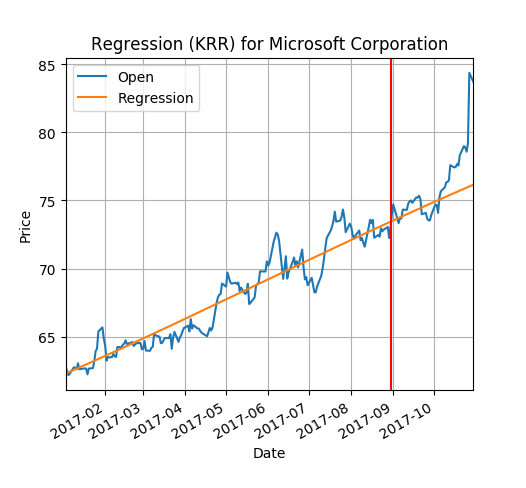
\includegraphics[width=150mm]{pictures/plots/microsoft_krr_80.png}
\caption{Wykres regresji grzbietowej dla 80\% danych uczących, Microsoft}
\label{fig:microsoft_krr_80}
\end{figure}

Wykres przedstawiający wyniki regresji grzbietowej dla największej ilości zastosowanych danych testowych przedstawia krzywą regresji zbliżoną kształtem do prostej.
Może to być spowodowane zastosowaniem zbyt dużej ilości danych uczących, które znajdują się w wyraźnym wzrostowym trendzie o niewielkich odchyleniach.\\

\subsection{Regresja Wektorów Nośnych}

Rysunki \ref{fig:microsoft_svr_20}, \ref{fig:microsoft_svr_50} i \ref{fig:microsoft_svr_80} przedstawiają wykresy wyników regresji wektorów nośnych dla wskazanego zbioru danych, 
o podziale danych uczących względem danych testowych odpowiednio: 20\%, 50\% i 80\%.\\

\begin{figure}[h!]
\centering
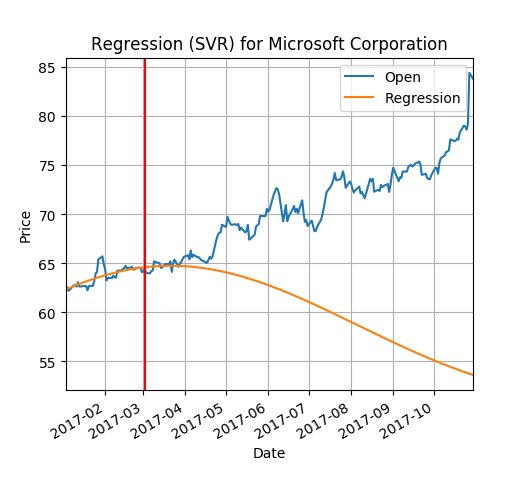
\includegraphics[width=150mm]{pictures/plots/microsoft_svr_20.png}
\caption{Wykres regresji wektorów nośnych dla 20\% danych uczących, Microsoft}
\label{fig:microsoft_svr_20}
\end{figure}

W powyższym przypadku regresja wektorów nośnych wykazuje bardzo niewielkie zdolności predykcyjne, a także niewielkie dopasowanie modelu.
Krzywa regresji po osiągnięciu granicy danych uczących, znacząco odchyla się w kierunku dolnym, coraz bardziej zwiększając błąd predykcji.\\

\begin{figure}[h!]
\centering
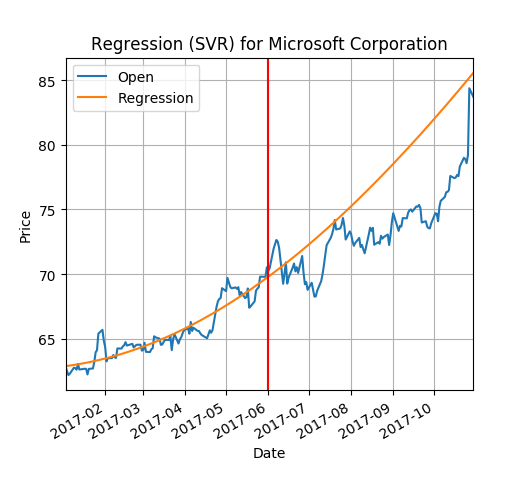
\includegraphics[width=150mm]{pictures/plots/microsoft_svr_50.png}
\caption{Wykres regresji wektorów nośnych dla 50\% danych uczących, Microsoft}
\label{fig:microsoft_svr_50}
\end{figure}

W odróżnieniu od krzywej regresji na rysunku \ref{fig:microsoft_svr_20}, w powyższym przypadku krzywa ta poprawnie przewiduje trend wzrostowy.
Jednakże odchylenie krzywej w stronę górną jest tak silne, że wraz ze wzrostem wartości na osi X wykresu, spada dopasowanie danych.\\

\begin{figure}[h!]
\centering
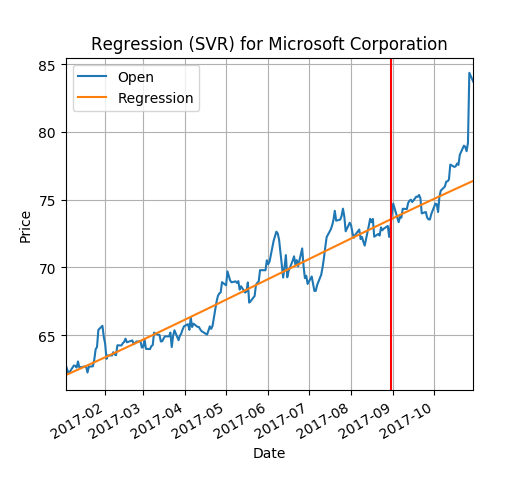
\includegraphics[width=150mm]{pictures/plots/microsoft_svr_80.png}
\caption{Wykres regresji wektorów nośnych dla 80\% danych uczących, Microsoft}
\label{fig:microsoft_svr_80}
\end{figure}

Na wykresie \ref{fig:microsoft_svr_80} można zaobserwować krzywą regresji wektorów nośnych, która przyjmuje postać prostej.
Zachowanie to jest zbieżne z zaobserwowanym na wykresach regresji grzbietowej, co może prowadzić do umocnienia wniosku o użytej zbyt dużej ilości danych uczących przy fakcie, iż dane te reprezentują silny trend wzrostowy.\\

\subsection{Regresja Procesu Gaussa}

Rysunki \ref{fig:microsoft_gpr_20}, \ref{fig:microsoft_gpr_50}, \ref{fig:microsoft_gpr_80} przedstawiają wykresy wyników analiz regresji procesu Gaussa dla odpowiednio: 20\%, 50\% i 80\% zastosowanych danych uczących.\\

\begin{figure}[h!]
\centering
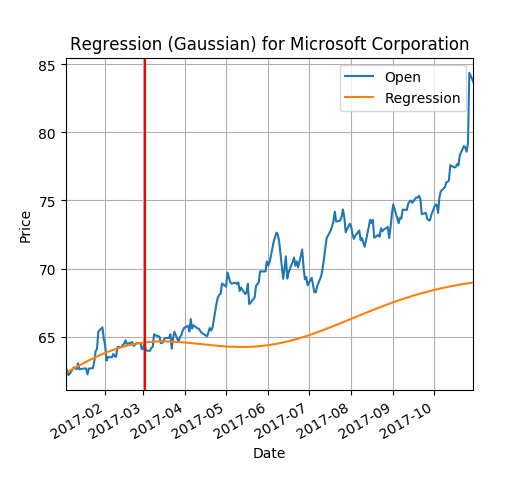
\includegraphics[width=150mm]{pictures/plots/microsoft_gpr_20.png}
\caption{Wykres regresji procesu Gaussa dla 20\% danych uczących, Microsoft}
\label{fig:microsoft_gpr_20}
\end{figure}

Na powyższym wykresie możemy zaobserwować zachowanie się krzywej regresji, które jest bardzo podobne do tej z rysunku \ref{fig:microsoft_svr_20}.
Spowodowane to może być zbyt małą ilością użytych danych uczących, które charakteryzują się niewielką zmiennością.\\

\begin{figure}[h!]
\centering
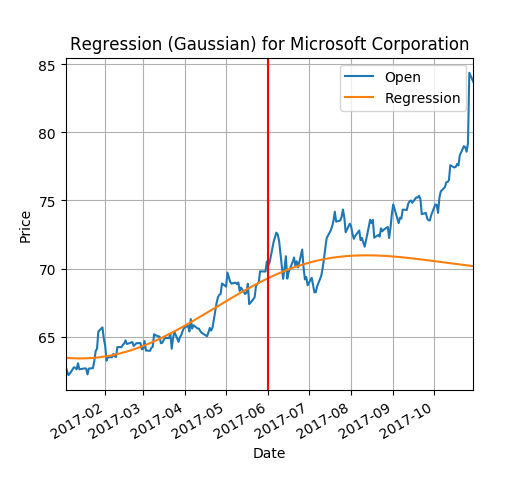
\includegraphics[width=150mm]{pictures/plots/microsoft_gpr_50.png}
\caption{Wykres regresji procesu Gaussa dla 50\% danych uczących, Microsoft}
\label{fig:microsoft_gpr_50}
\end{figure}

Wykres na rysunku \ref{fig:microsoft_gpr_50} powtarza tendencję z wykresu na rysunku \ref{fig:microsoft_gpr_20}.
Trend wzrostowy jest poprawnie przewidywany jedynie dla początkowych wartości danych testowych, a następnie występuje odchylenie krzywej regresji w dół.\\

\begin{figure}[h!]
\centering
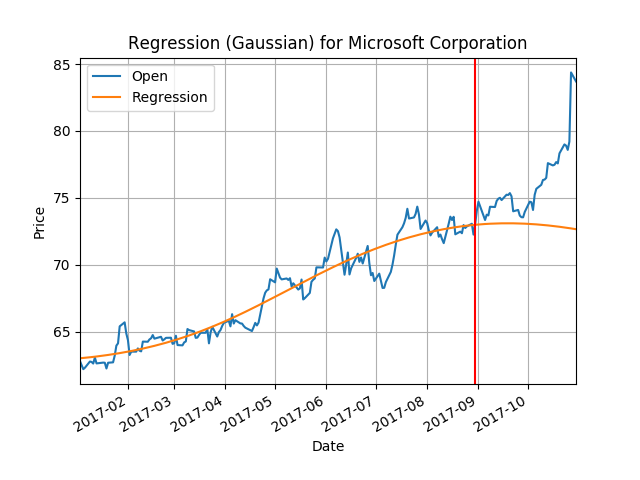
\includegraphics[width=150mm]{pictures/plots/microsoft_gpr_80.png}
\caption{Wykres regresji procesu Gaussa dla 80\% danych uczących, Microsoft}
\label{fig:microsoft_gpr_80}
\end{figure}

Krzywa regresji na powyższym wykresie w odróżnieniu od pozostałych nieliniowych metod regresji, nie wykazuje tendencji do zbliżania się kształtem do prostej.
Jednak predykcja dla zbioru testowego, oraz trend jaki wskazuje krzywa, gorzej odzwierciedlają rzeczywiste dane.\\

\subsection{Podsumowanie}

Podczas dokonanych analiz zebrano dane odnośnie wartości średniego błędu kwadratowego każdej z nich, a także wyniku predykcji. Przedstawiono je na wykresach znajdujących się na rysunkach \ref{fig:microsoft_mean_square} i \ref{fig:microsoft_score}.\\

\begin{figure}[h!]
\centering
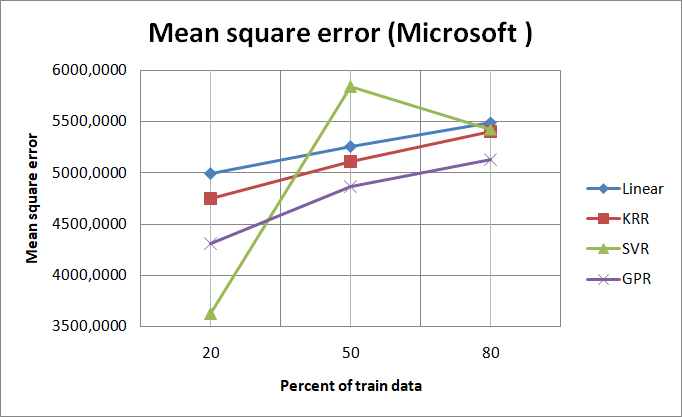
\includegraphics[width=150mm]{pictures/plots/microsoft_mean_square.png}
\caption{Wykres zmian wartości średniego błędu kwadratowego, Microsoft}
\label{fig:microsoft_mean_square}
\end{figure}

\begin{figure}[h!]
\centering
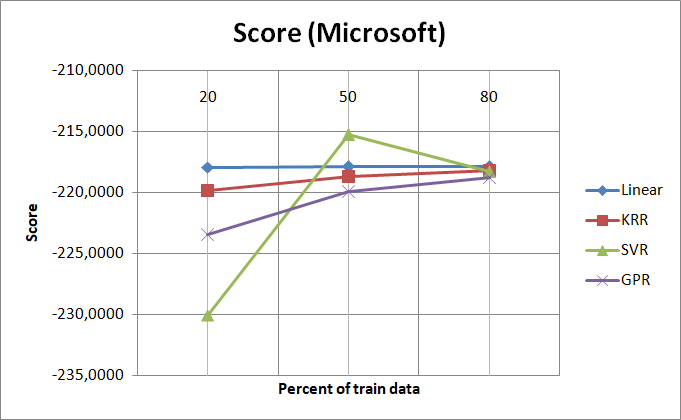
\includegraphics[width=150mm]{pictures/plots/microsoft_score.png}
\caption{Wykres zmian wartości wyników dopasowania modelu, Microsoft}
\label{fig:microsoft_score}
\end{figure}

Z powyższych wykresów wynika, iż średni błąd kwadratowy rośnie wraz ze wzrostem ilości danych uczących zastosowanych w analizie.
Wynik predycji natomiast odznacza się niewielkim wzrostem wraz ze zwiększaną ilością danych uczących.\\

Dla 20\% zastosowanych danych uczących najmniejszy błąd osiągnęła regresja wektorów nośnych, zaś największy - liniowa.
W przypadku wyniku predykcji jest natomiast odwrotnie: najlepszą wartość osiągnęła regresja liniowa,  a najgorszą regresja wektorów nośnych.\\

Dla 50\% zastosowanych danych uczących najmniejszym błędem kwadratowym charakteryzuje się regresja procesu Gaussa, a najwyższym regresja wektorów nośnych.
Powtórzona zostaje zależność zidentyfikowana w przypadku 20\% danych uczących: wynik predykcji oceniany najlepiej należy do regresji wektorów nośnych, natomiast najgorzej do regrtesji procesu Gaussa\\

W przypadku 80\% zastosowanych danych testowych regresja procesu Gaussa osiągnęła najniższy wynik średniego błędu kwadratowego. Pozostałe modele regresji charakteryzują się zbliżonym wynikiem.
Wynik predykcji dla każdego z modeli jest w tym przypadku bardzo zbliżony.\\

Na podstawie zgromadzonych wykresów, a także powyższych danych, można określić następujące wnioski:
\begin{itemize}
 \item trafne określenie trendu dla danych testowych zaobserwowano w przypadkach regresji liniowej, wektorów nośnych (80\% danych uczących) oraz grzbietowej (20\% i 80\% danych uczących)
 \item krzywe regresji, które nie identyfikowały poprawnie trendu dla danych testowych należą do regresji wektorów nośnych (20\% danych testowych) oraz procesu Gaussa
 \item w przypadku regresji grzbietowej (50\% danych uczących), zaobserwowano dobre dopasowanie i potwierdzenie trendu dla około 80\% danych testowych, po czym następowała zmiana nachylenia krzywej
\end{itemize}


\section{Testy zbioru danych: Intel}

\subsection{Informacje ogólne}
Zakres danych użytych do testów wynosi 81 próbek, w przedziale dat od 2017-01-01 do 2017-14-30 z krokiem wynoszącym jeden dzień.\\
Zakres ten charakteryzuje się mniejszą ilością danych o większej zmienności, niż zakres poprzedni.

\begin{figure}[h!]
\centering
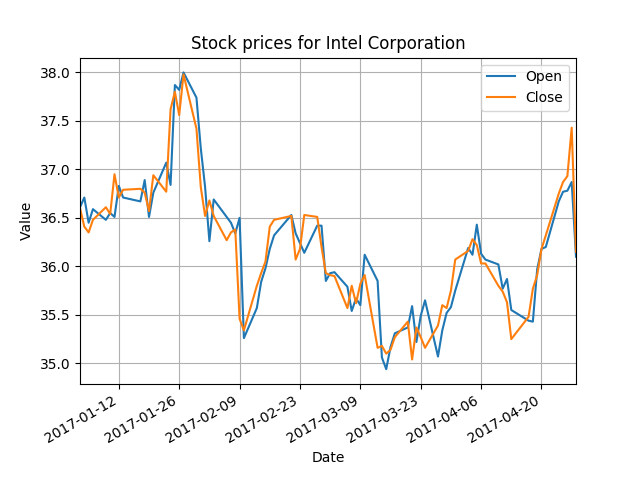
\includegraphics[width=150mm]{pictures/plots/intel_oc_price.png}
\caption{Wykres cen otwarcia i zamknięcia firmy Intel}
\label{fig:intel_oc_price}
\end{figure}

Na rysunku \ref{fig:intel_oc_price} przedstawiono wykres zmian cen otwarcia i zamknięcia dla podanego zakresu dat.\\ 

Ilość próbek danych uczących i testowych wynosi odpowiednio:
\begin{itemize}
 \item 16/65 dla wartości 20\% danych uczących
 \item 40/41 dla wartości 50\% danych uczących
 \item 64/17 dla wartości 80\% danych uczących
\end{itemize}

\subsection{Regresja liniowa}

Na wykresach \ref{fig:intel_linear_20}, \ref{fig:intel_linear_50} oraz \ref{fig:intel_linear_80} przedstawiono wyniko regresji liniowej o udziale danych uczących odpowiednio: 20\%, 50\% i 80\%.\\

\begin{figure}[h!]
\centering
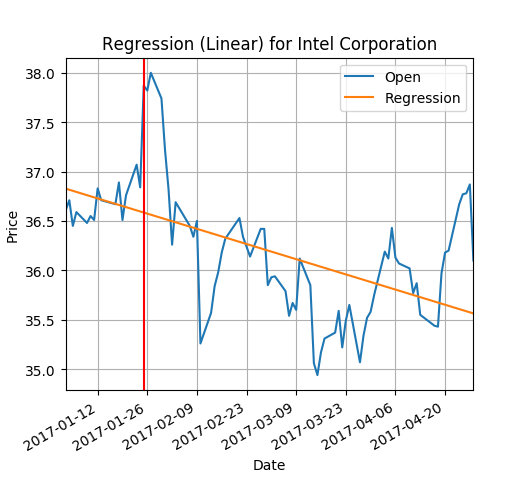
\includegraphics[width=150mm]{pictures/plots/intel_linear_20.png}
\caption{Wykres regresji liniowej dla 20\% danych uczących, Intel}
\label{fig:intel_linear_20}
\end{figure}

Z powyższego wykresu wynika, iż poprzez predykcję poprawnie zidentyfikowano trend spadkowy.\\

\begin{figure}[h!]
\centering
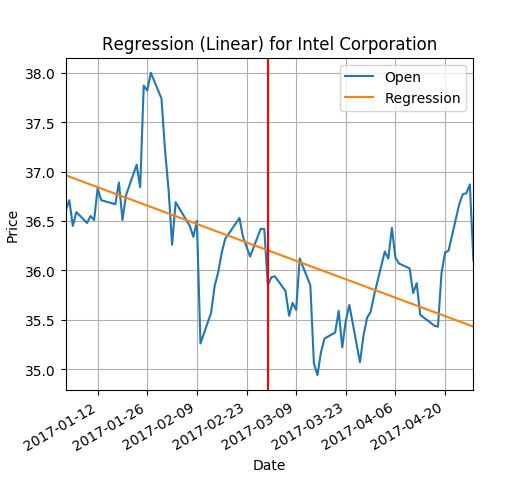
\includegraphics[width=150mm]{pictures/plots/intel_linear_50.png}
\caption{Wykres regresji liniowej dla 50\% danych uczących, Intel}
\label{fig:intel_linear_50}
\end{figure}

W porównaniu do wykresu na rysunku \ref{fig:intel_linear_50}, na powyższym wykresie zaobserwować można prostą regresji identyfikującą trend spadkowy, lecz o mniejszym nachyleniu niż poprzednio.
Może być to spowodowane lepszym dopasowaniem modelu, lub też zwiększoną liczbą danych uczących.\\

\begin{figure}[h!]
\centering
\includegraphics[width=150mm]{pictures/plots/intel_linear_80.png}
\caption{Wykres regresji liniowej dla 80\% danych uczących, Intel}
\label{fig:intel_linear_80}
\end{figure}

Porównując wszystkie trzy powyższe analizy regresji liniowej, można zaobserwować zależność spadku nachylenia prostej regresji od ilości zastosowanych danych uczących.

\subsection{Regresja Grzbietowa}

Na rysunkach \ref{fig:intel_krr_20}, \ref{fig:intel_krr_50} i \ref{fig:intel_krr_80} przedstawiono wyniko analizy regresji grzbietowej, przy zastosowaniu 20\%, 50\% i 80\% danych uczących.\\

\begin{figure}[h!]
\centering
\includegraphics[width=150mm]{pictures/plots/intel_krr_20.png}
\caption{Wykres regresji grzbietowej dla 20\% danych uczących, Intel}
\label{fig:intel_krr_20}
\end{figure}

Powyższy wykres wykazuje błędną predykcję i rozpoznanie trendu, które mogą być skutkiem zbyt małej ilości danych uczących.
Poza tym, dane zakres danych testowych obejmuje jedynie mniejszy trend wzrostowy, przez co utrudniona lub niemożliwa jest identyfikacja szerszego trendu spadkowego.\\

\begin{figure}[h!]
\centering
\includegraphics[width=150mm]{pictures/plots/intel_krr_50.png}
\caption{Wykres regresji grzbietowej dla 50\% danych uczących, Intel}
\label{fig:intel_krr_50}
\end{figure}

Wykres \ref{fig:intel_krr_50} przedstawia krzywą regresji, która charakteryzuje się dobrym dopasowaniem w części danych uczących, lecz w części danych testowych staje się ona niemal linią prostą.
Może być to ponownie spowodowane nietrafnie dobranym zakresem danych uczących, ponieważ można w nim zaobserwować zarówno duży wzrost i duży spadek, co w połączeniu z małą ilością próbek danych może czynić zbiór niereprezentacyjnym.\\

\begin{figure}[h!]
\centering
\includegraphics[width=150mm]{pictures/plots/intel_krr_80.png}
\caption{Wykres regresji grzbietowej dla 80\% danych uczących, Intel}
\label{fig:intel_krr_80}
\end{figure}

Spośród trzech przedstawionych analiz regresji grzbietowej, wykres na rysunku \ref{fig:intel_krr_80} zdecydowanie przedstawia krzywą regresji najlepiej przedstawiającą trend.
Należy jednak zauważyć, iż fragment przedstawiający dane testowe jest relatywnie niewielki, a przewidywane wartości nie pokrywają się w żadnym punkcie z wartościami testowymi.\\

\subsection{Regresja Wektorów Nośnych}

Rysunki \ref{fig:intel_svr_20}, \ref{fig:intel_svr_50} i \ref{fig:intel_svr_80} przedstawiają wykresy analizy regresji wektorów nośnych dla proporcji danych uczących wynoszących odpowiednio: 20\%, 50\% i 80\%.\\

\begin{figure}[h!]
\centering
\includegraphics[width=150mm]{pictures/plots/intel_svr_20.png}
\caption{Wykres regresji wektorów nośnych dla 20\% danych uczących, Intel}
\label{fig:intel_svr_20}
\end{figure}

Powyższy wykres przedstawia podobną zależność, co wykres analizy regresji grzbietowej dla tych samych ilości danych uczących.
Podtrzymany zostaje więc wniosek, iż niepoprawna identyfikacja trendu spowodowana może być złym dobraniem danych uczących, reprezentujących jedynie mniejszy trend wzrostowy.\\

\begin{figure}[h!]
\centering
\includegraphics[width=150mm]{pictures/plots/intel_svr_50.png}
\caption{Wykres regresji wektorów nośnych dla 50\% danych uczących, Intel}
\label{fig:intel_svr_50}
\end{figure}

Wykres na rysunku \ref{fig:intel_svr_50} wykazuje poprawne dopasowanie modelu regresji w części danych uczących, lecz w części danych testowych błędnie identyfikuje trend, a krzywa regresji przybiera postać prostej.
Może to być spowodowane błędnym dobraniem parametrów obiektu \textit{SVR()}.\\

\begin{figure}[h!]
\centering
\includegraphics[width=150mm]{pictures/plots/intel_svr_80.png}
\caption{Wykres regresji wektorów nośnych dla 80\% danych uczących, Intel}
\label{fig:intel_svr_80}
\end{figure}

Podobnie jak w przypadku wykresu \ref{fig:intel_krr_80} regresji grzbietowej, także i w powyższym przypadku dopasowanie modelu i identyfikacja trendu spadkowego są zauważalne.\\

\subsection{Regresja Procesu Gaussa}

Na rysunkach \ref{fig:intel_gpr_20}, \ref{fig:intel_gpr_50} i \ref{fig:intel_gpr_80} przedstawiono wykresy analizy regresji procesu Gaussa dla następujących ilości danych testowych: 20\%, 50\% i 80\%.\\

\begin{figure}[h!]
\centering
\includegraphics[width=150mm]{pictures/plots/intel_gpr_20.png}
\caption{Wykres regresji procesu Gaussa dla 20\% danych uczących, Intel}
\label{fig:intel_gpr_20}
\end{figure}

W powyższym przypadku krzywa regresji poprawnie identyfikuje trend spadkowy w części testowej, jednakże niewielkie nachylenie krzywej nie oddaje do końca charakteru spadkowego danych.\\ 

\begin{figure}[h!]
\centering
\includegraphics[width=150mm]{pictures/plots/intel_gpr_50.png}
\caption{Wykres regresji procesu Gaussa dla 50\% danych uczących, Intel}
\label{fig:intel_gpr_50}
\end{figure}

Na rysunku \ref{fig:intel_gpr_50} można zaobserwować krzywą regresji poprawnie opisującą i przewidującą przebieg trendu.
W części danych testowych zauważalny jest nie tylko delikatny spadek, lecz również wzrost dla końcowych wartości danych, co zgadza się z wartościami testowymi.\\

\begin{figure}[h!]
\centering
\includegraphics[width=150mm]{pictures/plots/intel_gpr_80.png}
\caption{Wykres regresji procesu Gaussa dla 80\% danych uczących, Intel}
\label{fig:intel_gpr_80}
\end{figure}

W porównaniu do poprzednich wyników regresji procesu Gaussa, powyższy wykres potwierdza wniosek, iż wraz ze wzrostem ilości danych testowych dla tego zbioru danych, rośnie dopasowanie modelu oraz jakość predykcji.\\

\subsection{Podsumowanie}

Dane dotyczące średniego błędu kwadratowego oraz wyników predykcji modeli regresji są przedstawione na wykresach \ref{fig:intel_mean_square} oraz \ref{fig:intel_score}.\\

\begin{figure}[h!]
\centering
\includegraphics[width=150mm]{pictures/plots/intel_mean_square.png}
\caption{Wykres zmian wartości średniego błędu kwadratowego, Intel}
\label{fig:intel_mean_square}
\end{figure}

\begin{figure}[h!]
\centering
\includegraphics[width=150mm]{pictures/plots/intel_score.png}
\caption{Wykres zmian wartości wyników dopasowania modelu, Intel}
\label{fig:intel_score}
\end{figure}

Z powyższych danych wynika, iż dla ilości danych uczących wynoszącej 20\% najwyższy średni błąd kwadratowy uzyskały modele regresji wektorów nośnych oraz grzbietowa, najniższy zaś model regresji liniowej.
Dla ilości danych uczących wynoszącej 50\% najwyższa wartość błędu odnosi się do modelu regresji wektorów nośnych, a najniższa do modelu regresji liniowej.
Dla 80\% danych uczących natomiast, wszystkie modele regresji osiągnęły podobną, niską wartość, z wyjątkiem modelu regresji procesu Gaussa, który osiągnął wartość najwyższą.\\

W odróżnieniu od poprzedniego testowanego zakresu danych, w tym przypadku zaobserwować można tendencję spadku wartości średniego kwadratu błędów wraz ze wzrostem procentowej ilości użytych danych uczących.\\

Z wykresu \ref{fig:intel_score} wynika, iż wraz ze wzrostem ilości użytych danych uczących spada wartość dopasowania każdego modelu, z wyjątkiem modelu liniowego, który przedstawia za każdym razem podobną wartość.
Może być to spowodowane faktem, iż wartość ta jest liczona jedynie dla danych testowych, więc przy zmniejszaniu ich ilości obserwujemy spadek dopasowania.\\

Analiza wykresów pozwala wnioskować, iż trafne określenie trendu można dostrzec na wykresach regresji procesu Gaussa, liniowej, grzbietowej (80\% danych uczących) oraz wektorów nośnych (80\% danych uczących).
Natomiast niedokładna predykcja trendu widoczna jest na wykresach regresji grzbietowej (20\% i 50\% danych uczących) oraz wektorów nośnych (20\% i 50\% danych uczących).\\

\section{Wnioski}

\begin{enumerate}
 \item Dokładność predykcji modelu regresji liniowej zmienia się nieznacznie w zależności od zmiany proporcji ilości danych uczących względem danych testowych.
 \item Przedstawione modele regresji nieliniowych wykazują dużą wrażliwość na wysoką zmienność danych poddawanych analizie, przez co w celu osiągnięcia bardziej dokładnych wyników predykcji niezbędne jest znalezienie właściwych zakresów parametrów podawanych jako argumenty do obiektów tych regresji.
 \item Wartości średniego kwadratu błędów oraz wyników predykcji (dopasowania modelu) wykazują zależność od całkowitej ilości analizowanych danych. Wraz ze wzrostem ich ilości zwiększają się wartości błędów, a wyniki predykcji ulegają polepszeniu.
 \item Dobre właściwości określania trendu dla obydwu testowanych zakresów danych wykazały: regresja liniowa, wektorów nośnych (przy 80\% danych uczących) oraz grzbietowa (przy 80\% danych uczących).
 \item Regresja procesu Gaussa w przypadku dużego zbioru danych nie wykazała dobrych zdolności predykcyjnych, natomiast w przypadku małego zbioru można ją uznać za najlepszą metodę regresji dla podanych warunków.
 \item Jakość predykcji za pomocą testowanych metod w dużym stopniu zależy od struktury danych użytych do analizy. Jednocześnie najbardziej odporną na ten czynnik metodą okazała się regresja liniowa.
 \item Wraz ze wzrostem ilości użytych do analizy danych uczących, w większości przypadków wzrasta trafność predykcji lub trafność określenia trendu.
 \item Pakiet \textit{Scikit-learn} i udostępniane przez niego metody regresji są przydatne w analizie danych giełdowych. Ich dokładność można zwiększyć odpowiednio parametryzując tworzone obiekty modeli regresji, oraz poprawnie dobierając dane.
\end{enumerate}



%%% ------- ROZDZIAŁ 5 ------- %%

\chapter{Wnioski}



%% ------- ZAKOŃCZENIE ------- %%
%%
% \begin{zakonczenie}  % ew. np. \begin{zakonczenie}[Podsumowanie]
%%
%
%  <Treść zakończenia, podsumowania (jeśli jest taka potrzeba umieszczenia)>
%
%%
% \end{zakonczenie}
%%
%%
%% -----------------------
%%   ROZDZIAŁY DODATKOWE
%% -----------------------
%%
% \appendix
%%
%% ------- DODATEK A ------- %%
%%
% \chapter{----}
%%
%
%  <Treść dodatku A, może być umieszczona w innym pliku
%   i ładowana przez \input{----} lub \includeonly{...,...}>
%
%%
%%
%% ----------------
%%   BIBLIOGRAFIA
%% ----------------
%%
%  (Możemy użyć środowiska 'thebibliography' lub też bazy BiBTeX)
%%
%% BiBTeX (opcjonalnie)
% \bibliography{<pliki bib>}
%%
\begin{thebibliography}{88}  % ew. np. '8' jeśli liczba pozycji < 10
%% Przykładowe wrzuty

\bibitem{gpw} Tobiasz Maliński, 
\textit{Giełda Papierów Wartościowych Dla Bystrzaków}, Helion 2016.

\bibitem{basics_of_tech_analysis} Justin Kuepper,
\textit{Basics of Technical Analysis}, 19 Kwiecień 2017.
https://www.investopedia.com/university/technical/

\bibitem{stock_market} Investopedia,
\textit{Stock Market}, 20 Listopad 2017.\\
https://www.investopedia.com/terms/s/stockmarket.asp

\bibitem{ustawa_22_03_1991_papiery_wartosciowe} Prawo o publicznym obrocie papierami wartościowymi i funduszach powierniczych
\textit{Ustawa z dnia 22 marca 1991r.}, Art 2.

\bibitem{akcje} Roman Ciepiela, Piotr Pytlik, Magda Wiernusz,
\textit{Encyklopedia Zarządzania}\\
25 Październik 2016.\\
https://mfiles.pl/pl/index.php/Akcje

\bibitem{obligacje} Roman Ciepiela, Szymon Kułakowski, Sabina Blok,
\textit{Encyklopedia Zarządzania}, 13 Lipiec 2017
https://mfiles.pl/pl/index.php/Obligacje

\bibitem{ekonometria} Małgorzata Łuniewska
\textit{Ekonometria Finansowa: Analiza rynku kapitałowego}, Warszawa 2008
Wydawnictwo Naukowe PWN

\bibitem{tech_analysis_pillars} Stockopedia
\textit{Technical Analysis (Part 1): History, Theory and Philosophy}\\
Kwiecień 2017\\
https://www.stockopedia.com/content/technical-analysis-part-1-history-theory-and-philosophy-179598/

\bibitem{ekonometria_model} G.S. Maddala
\textit{Ekonometria} Warszawa 2006\\
Wydawnictwo Naukowe PWN

\bibitem{analiza_fundamentalna_techniczna} Mariusz Czekała
\textit{Analiza fundamentalna i techniczna} Wrocław 1997\\
Wydawnictwo Akademii Ekonomicznej im. Oskara Langego we Wrocławiu

\bibitem{systemy_uczace_sie} Jacek Koronacki, Jan Ćwik
\textit{Statystyczne Systemy Uczące Się} Warszawa 2005\\
Wydawnictwa Naukowo-Techniczne

\bibitem{decision_tree_classification} Emil Lundkvist
\textit{Decision Tree Classification and Forecasting of Pricing Time Series Data} Stockholm 2014\\
Master’s Degree Project

\bibitem{intro_machine_learning} Alex Smola
\textit{Introduction to Machine Learning} 2008\\
Cambridge University Press

\bibitem{bayes} Paweł Cichosz
\textit{Systemy Uczące Się} Warszawa 2000\\
Wydawnictwo Naukowo-Techniczne Warszawa

\bibitem{drzewa_decyzyjne} Mirosław Krzyśko
\textit{Systemy uczące się} Warszawa 2008
Wydawnicatwa Naukowo-Techniczne

\bibitem{statystyka} Stanisław M. Kot
\textit{Statystyka} Warszawa 2011
Difin SA

\bibitem{analiza_danych} Siegmund Brandt
\textit{Analiza Danych} Warszawa 1998
Wydawnictwo Naukowe PWN

\bibitem{learning_python} Fabrizio Romano
\textit{Learning Python} 2015
Packt Publishing

\bibitem{numpy_ug} NumPy Community
\textit{NumPy User Guide} Release 1.13.0

\bibitem{scipy_doc} SciPy.org
\textit{SciPy Documentation}
https://docs.scipy.org/doc/scipy/reference/

\bibitem{scikit_article} Fabian Pedregosa
\textit{Scikit-learn: Machine Learning in Python}
Journal of Machine Learning Research 12 (2011

\bibitem{scikit_doc} scikit-learn.org
\textit{Sciki-learn Documentation}
http://scikit-learn.org/stable/documentation.html

\bibitem{mastering_stat} Gavin Hackeling
\textit{Mastering Machine Learning with scikit-learn}
Packt Publishing


%%
\end{thebibliography}
%%
%%
%% ----------------------------
%%   DODATKOWE ELEMENTY PRACY
%% ----------------------------
%%
%  Tutaj umieścimy dodatkowe (niebowiązkowe) cześci pracy:
%  - Spis skrótów, symboli i oznaczeń (jako \chapter*{...})
%  - Spis ilustracji (\listoffigures)
%  - Spis tablic (\listoftables)
%  - Skorowidz (nieobowiązkowy, umieszczenie ułatwia lekturę pracy)
%
% \chapter*{Spis symboli i oznaczeń}  % ew. podobny tytuł
%  
%   <Tabela ze spisem symboli, oznaczeń itp.>
%
\listoffigures
%
\listoftables
%
%\printindex  % jeżeli do pracy dołączony jest indeks
%%
%%
\end{document}
%%
%% [Wersja dla: 2011/09/06 v1.06]
%%====================================================================%%
